\chapter{Evolução do Sistema}

\section{Contexto Energético}
O crescimento no consumo de energia cada vez mais vem aumentando conforme os anos. No
ano de 2014 o Brasil consumiu 531.1 TWh, resultando em um aumento de 2.9\% comparado à 2013. Além disso, a matriz energética brasileira é predominantemente renovável, tendo como ênfase a geração hidráulica. As fontes renováveis correspondem à 84.1\% e não renováveis 26.9\% \cite{balanco_energetico}.

Uma pequena parte do consumo total de energia elétrica do Brasil é realizada por prédios públicos, sendo
esses responsáveis pela prestação de serviços à população. Em 2014, o total de energia elétrica consumida
pelos mesmos foi de 12.61 TWh, representando 2.4\% do total consumido pelo país \cite{balanco_energetico}.

No ano de 2015 foi realizado um reajuste tarifário da energia elétrica correspondente à 33\% para clientes residenciais e 32,5\% para empresas, indústrias e comércios \cite{aumento_energia}, gerando altos gastos.

Dentre as alternativas para reduzir o consumo de energia elétrica encontram-se o uso de equipamentos mais eficientes, certificações Procel\footnote{\url{www.procelinfo.com.br/selo_procel_edificacoes/}}, uso racional da energia e afins, porém, quando se trata de instalações de grande porte, como Universidades e órgãos públicos em geral, percebe-se que um dos grandes problemas enfrentado é a falta de monitoramento adequado do uso de energia elétrica.

Em Maio de 2016, a Prefeitura de Campus da Universidade de Brasília (UnB) aprovou um projeto de gerenciamento energético da própria Universidade, objetivando que cada Campus da instituição (Asa Norte, Ceilândia, Gama e Planaltina) seja responsável por realizar, com o auxílio de transdutores, seu próprio monitoramento de energia e enviar essas informações coletadas para o Campus Darcy Ribeiro. O sistema para auxiliar todo o projeto foi denominado Sistema de Monitoramento Energético - Universidade de Brasília (SME-UnB).

Este trabalho contribuiu com o desenvolvimento de uma parte do SME-UnB.

\section{Sprint 01 (25/07/2016 à 05/08/2016) - Coleta Inicial de Dados do Transdutor}
Buscando realizar uma primeira análise do transdutor instalado na Universidade, verificando se a comunicação com o mesmo poderia ser realizada de maneira efetiva, realizou-se o módulo \textit{data\_reader} contendo as seguintes classes:
\begin{itemize}
    \item Transductor: representação de um transdutor.
    \item Measurements: representação das medições de energia realizadas pelo transdutor.
    \item CommunicationProtocol: acoplamento dos protocolos de transporte e serial, visando realizar uma comunicação com o transdutor.
\end{itemize}

A figura \ref{sprint01arq} representa a arquitetura inicial do projeto, onde basicamente um transdutor possui várias medições de energia e, dependendo do seu modelo, pode possuir diferentes protocolos para se comunicar.

\begin{figure}[!htpb]
    \centering
    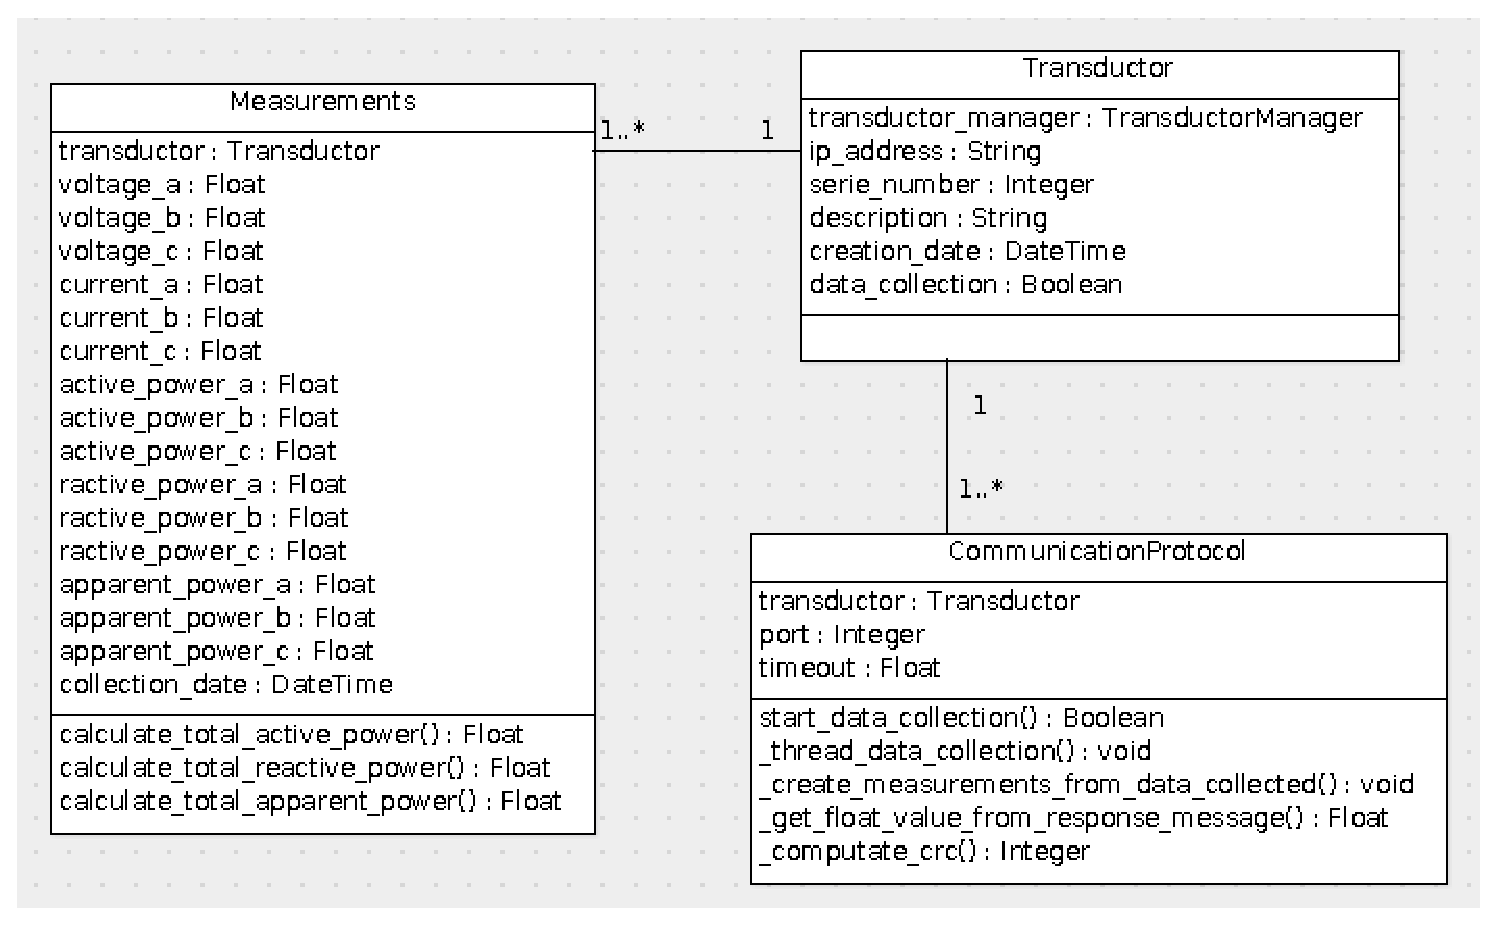
\includegraphics[keepaspectratio=true,scale=0.6]{figuras/sprint01arq.eps}
    \caption{Arquitetura SME-UnB \textit{Sprint 01}. Fonte: autor}
    \label{sprint01arq}
\end{figure}

\vfill
\pagebreak

Foram realizar algumas telas, figuras \ref{dados01} e \ref{dados02}, contendo os dados de energia coletados para apresentação ao usuário.

\begin{figure}[!htpb]
    \centering
    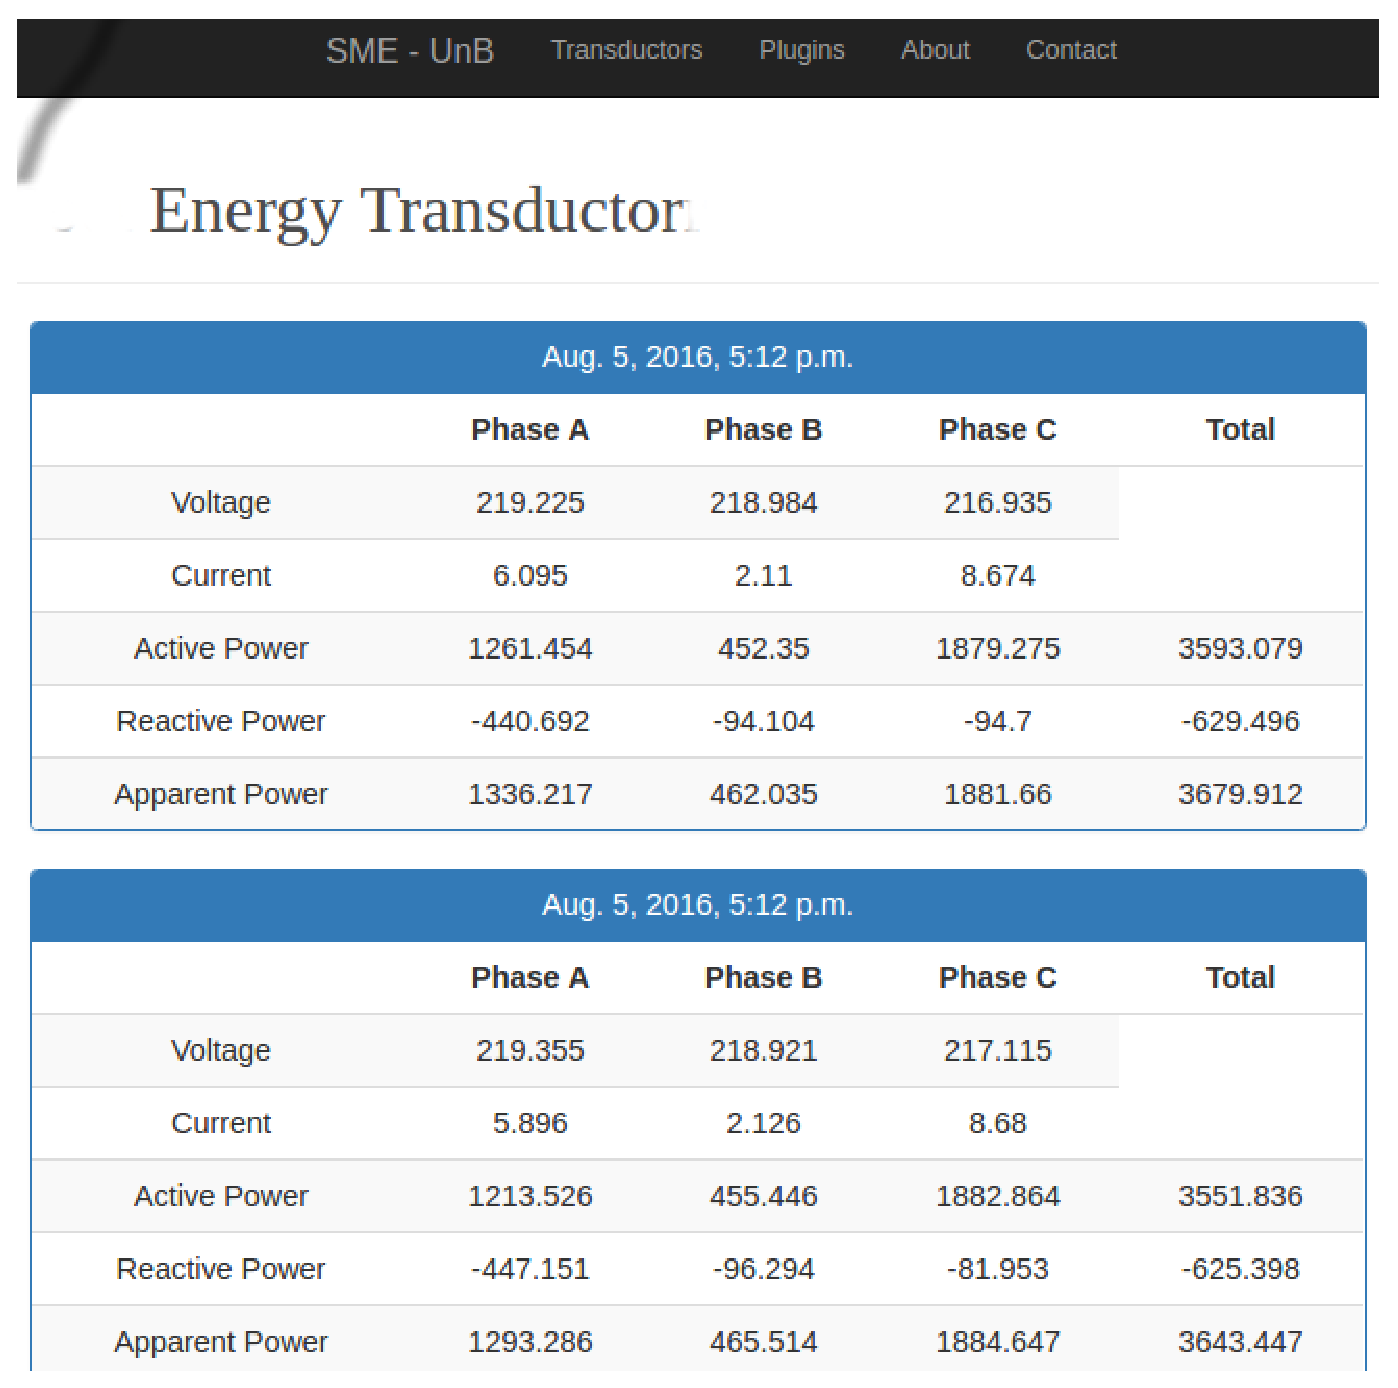
\includegraphics[keepaspectratio=true,scale=0.5]{figuras/coleta_dados_01.eps}
    \caption{Página apresentação medições de energia. Fonte: autor}
    \label{dados01}
\end{figure}

\begin{figure}[!htpb]
    \centering
    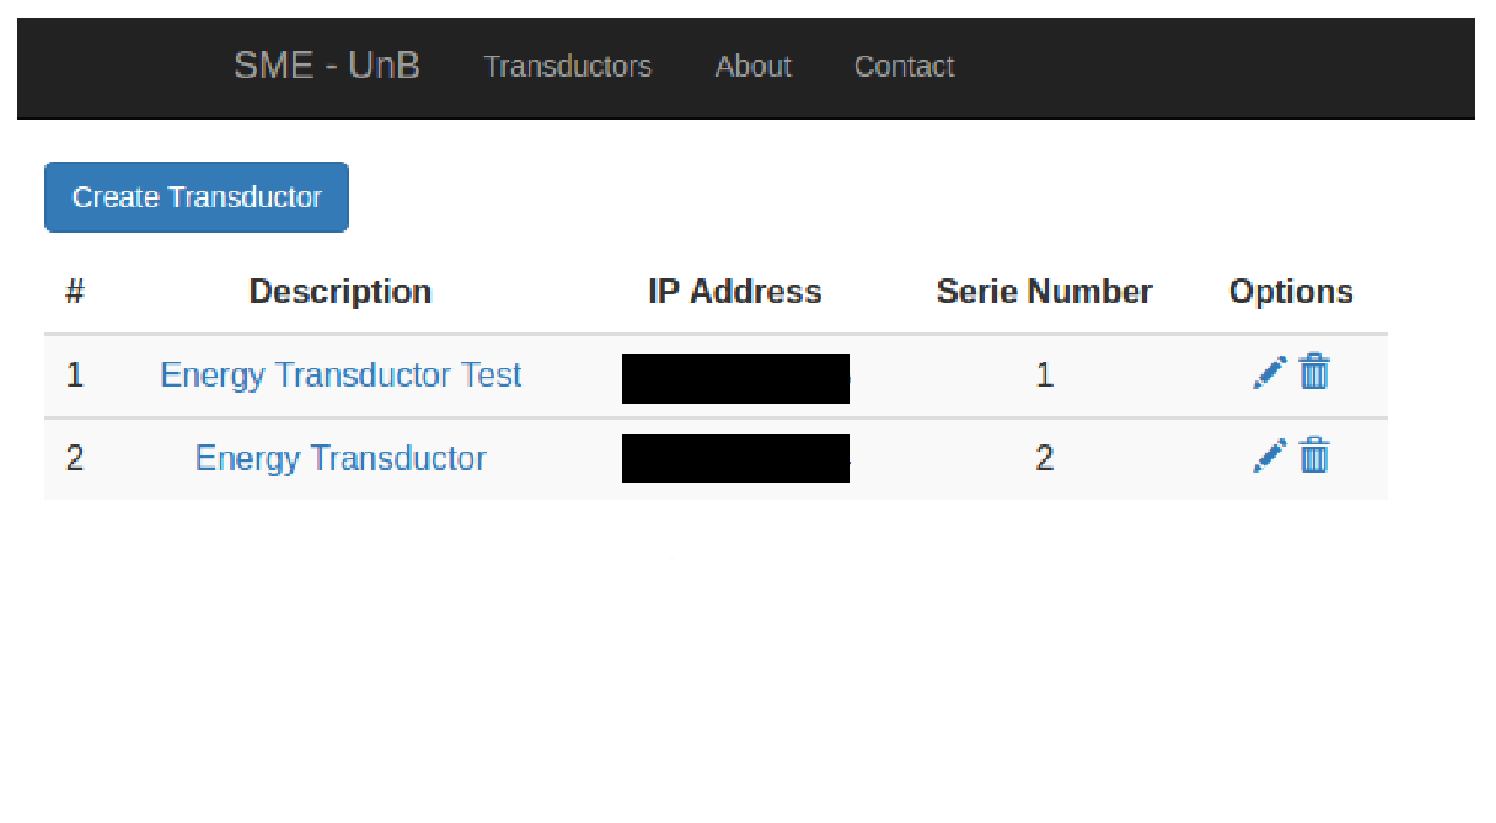
\includegraphics[keepaspectratio=true,scale=0.5]{figuras/coleta_dados_02.eps}
    \caption{Página apresentação medições de energia. Fonte: autor}
    \label{dados02}
\end{figure}

\vfill
\pagebreak

\section{Sprint 02 (08/08/2016 à 19/08/2016) - Refatorações de \textit{Urls}/\textit{Templates} e Guia de Instalação}
Após analisadas as \textit{urls} e \textit{templates} do projeto verificou-se que havia muitas rotas desnecessárias e não havia um padrão para os templates, o que estava gerando confusão na hora de criar novas páginas para a aplicação. Tendo em mente tais problemas essa sprint buscou realizar uma refatoração dos mesmos.

Realizou-se um guia de instalação\footnote{\url{https://gitlab.com/brenddongontijo/SME-UnB/wikis/instalation-guide/}} para o ambiente de desenvolvimento utilizando as ferramentas \textit{Vagrant}\footnote{\url{https://www.vagrantup.com/}} e \textit{Chef Solo}\footnote{\url{https://docs.chef.io/chef_solo.html}}, visando auxiliar novos desenvolvedores a contribuirem com o projeto.

\section{Sprint 03 (22/08/2016 à 02/09/2016) - Reestruturação Arquitetura e Primeiros Testes}
Realizou-se uma reunião com o orientador visando reestruturar a arquitetura. Primordialmente, tendo em vista que os tradutores podem possuir diferentes tipos de medições, foram definidas duas classes abstratas: Transductor e Measurements. A partir dessas classes surgiram as especializações de transdutores de energia (EnergyTransductor) e medições de energia (EnergyMeasurements). Além disso, percebeu-se a necessidade de criação de um modelo de transdutor (TransductorModel), o qual possuiria informações específicas do mesmo, como endereço dos registradores importantes, protocolo serial e de transporte utilizados. A figura \ref{sprint03arq} ilustra a evolução da arquitetura realizada nessa sprint.

\begin{figure}[!htpb]
    \centering
    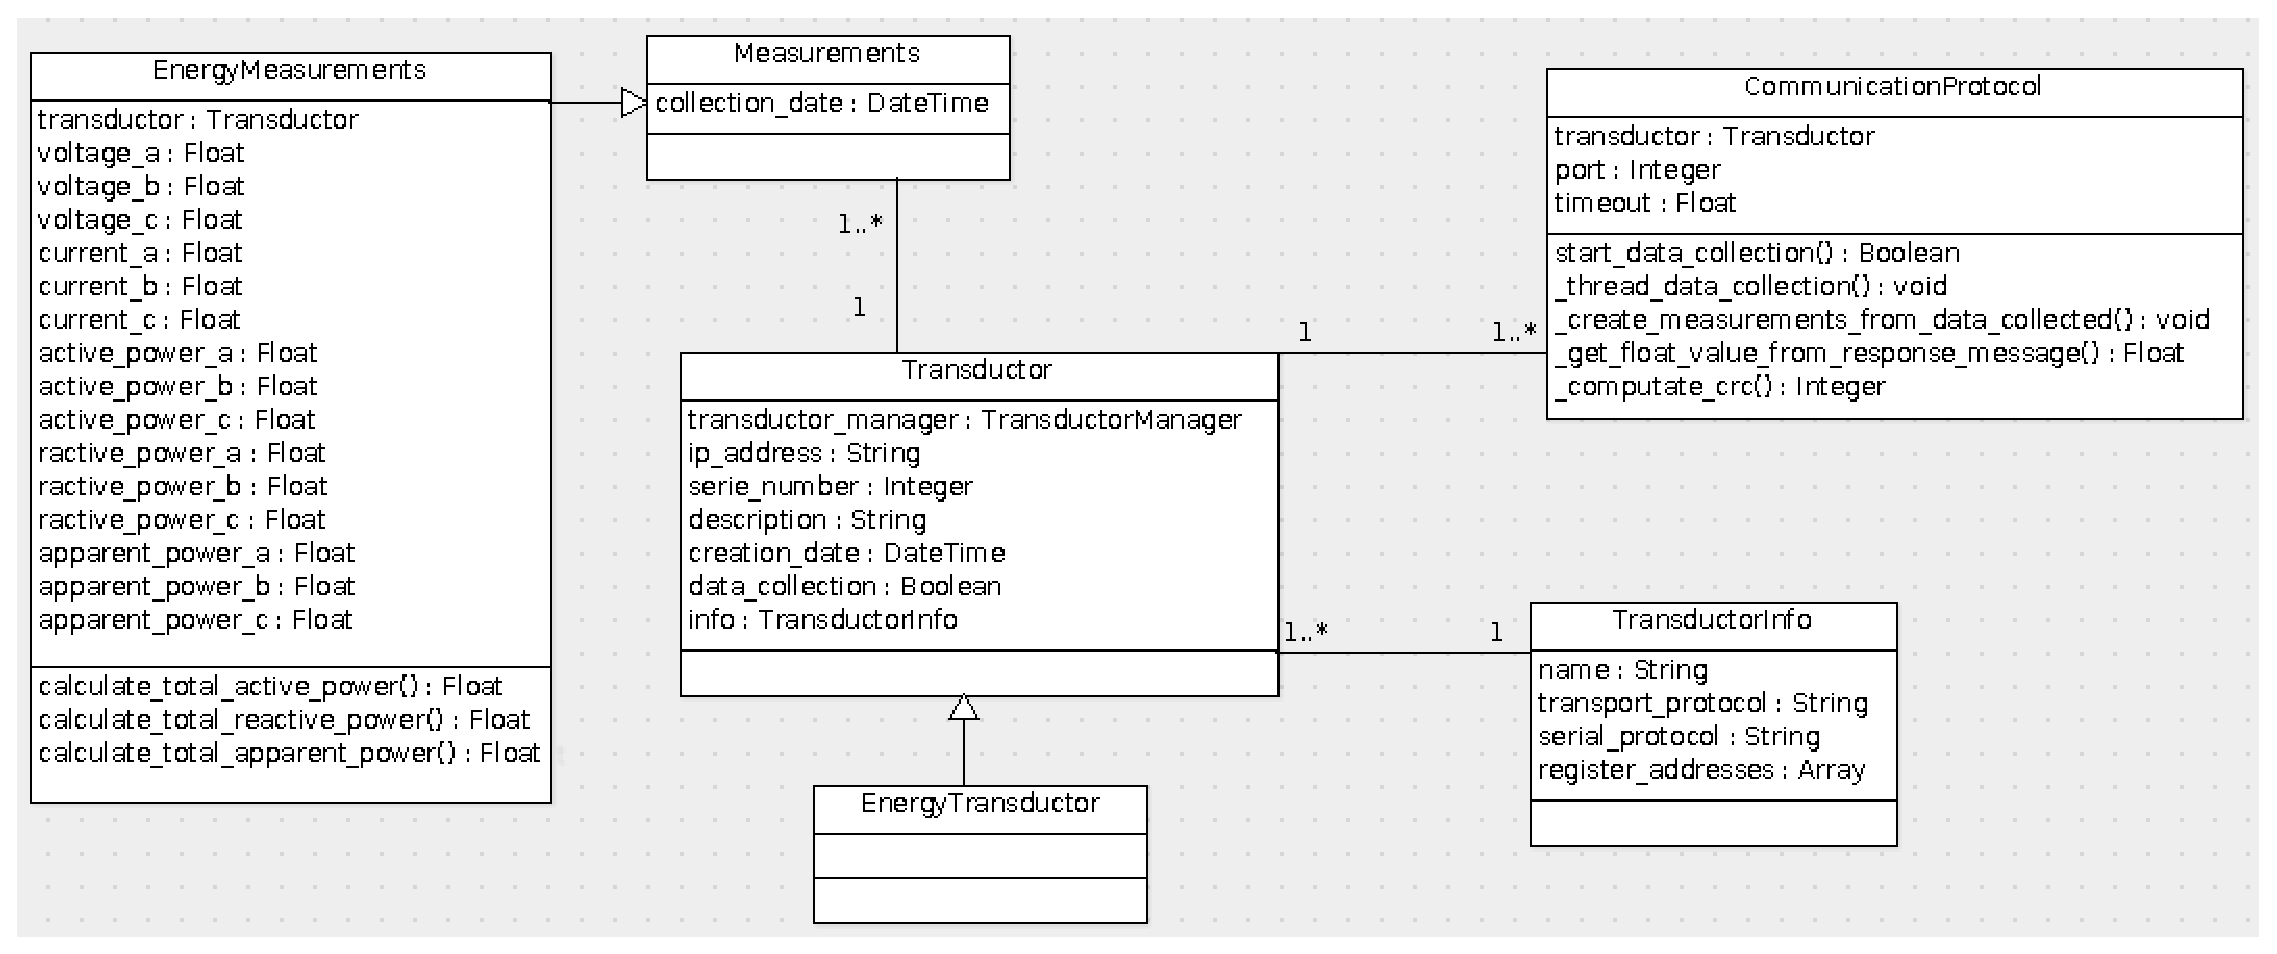
\includegraphics[scale=0.6,angle=90]{figuras/sprint03arq.eps}
    \caption{Arquitetura SME-UnB Sprint 03. Fonte: autor}
    \label{sprint03arq}
\end{figure}

\vfill
\pagebreak

Nessa sprint foi realizado um primeiro contato com os testes e ao seu fim obtivo-se uma cobertura de 71\%, conforme a figura \ref{cobertura01}.

\begin{figure}[!htpb]
    \centering
    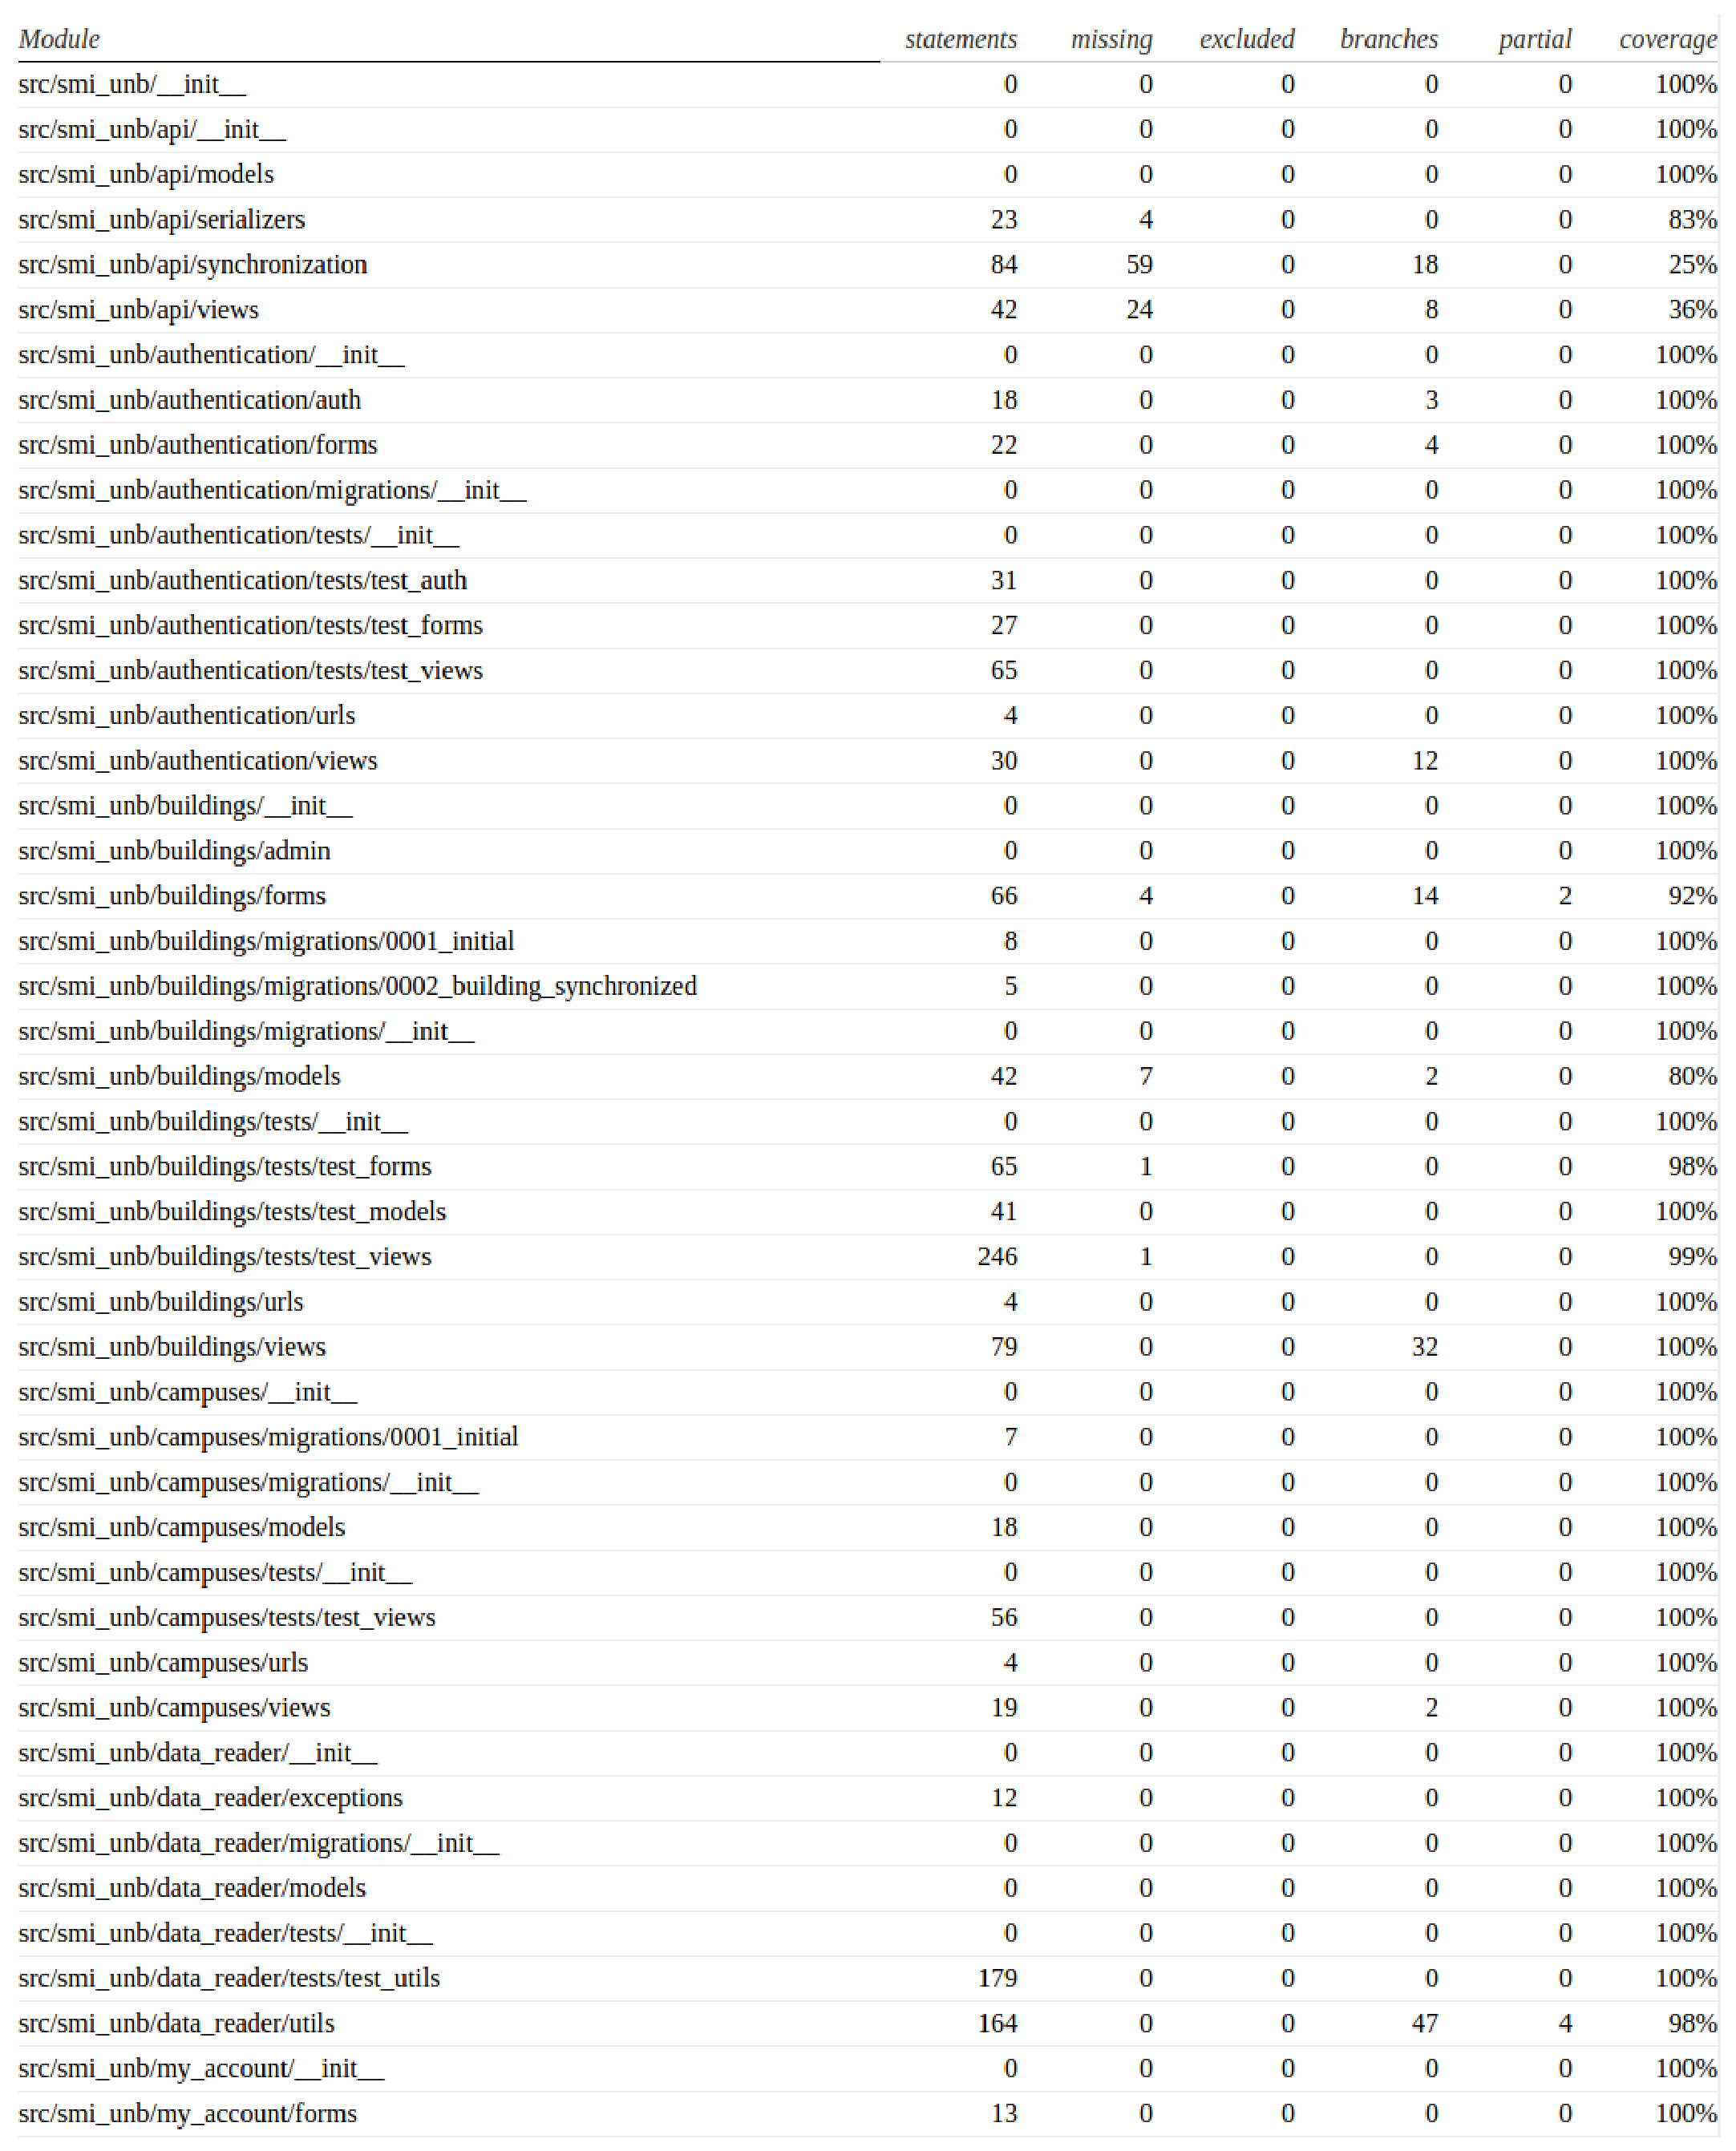
\includegraphics[keepaspectratio=true,scale=0.5]{figuras/cobertura01.eps}
    \caption{Cobertura Total de Código Sprint 03. Fonte: autor}
    \label{cobertura01}
\end{figure}

\section{Sprint 04 (05/09/2016 à 16/09/2016) - Documentação de Código e Estrutura \textit{Boilerplate}}
Buscando deixar o código mais entendível, realizou-se uma documentação das principais classes do sistema utilizando os padrões de \textit{docstrings}\footnote{\url{https://www.python.org/dev/peps/pep-0257/}} definidos pelo \textit{Google Python Style}\footnote{\url{http://google.github.io/styleguide/pyguide.html}}. A figura \ref{documentacao01} ilustra um exemplo realizado no projeto.

\begin{figure}[!htpb]
    \centering
    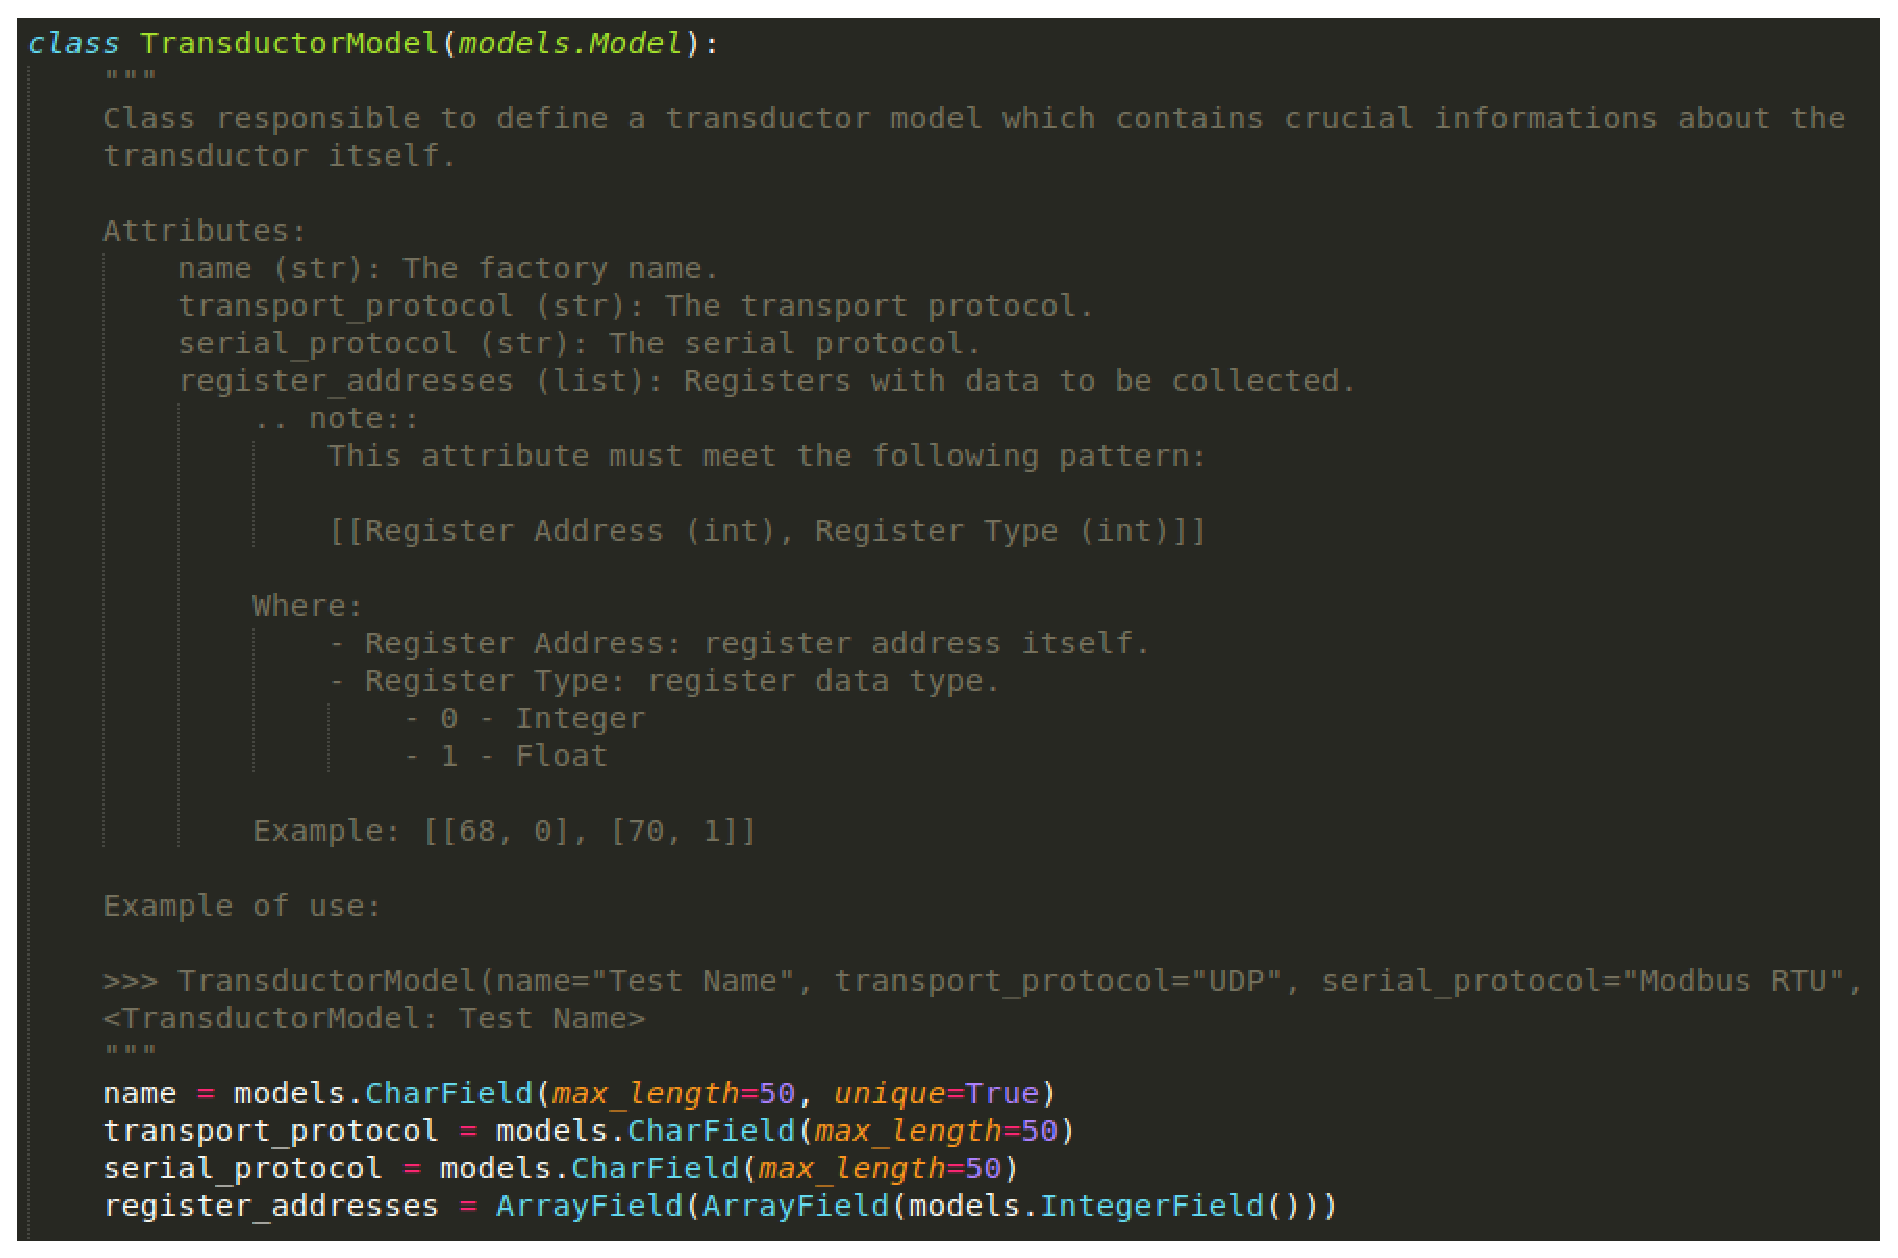
\includegraphics[keepaspectratio=true,scale=0.5]{figuras/documentacao01.eps}
    \caption{Exemplo de Documentação Utilizando \textit{Google Python Style}. Fonte: autor}
    \label{documentacao01}
\end{figure}

A estrutura \textit{Boilerplate}\footnote{\url{https://github.com/fabiommendes/python-boilerplate}} foi adicionada ao projeto com o objetivo de realizar uma melhor estruturação dos módulos e realizar pré-configurações para ambientes de desenvolvimendo/produção, assim como no auxílio para utilização das ferramentas \textit{Sphinx} e \textit{Coverage}.

\section{Sprint 05 (19/09/2016 à 30/09/2016) - Refatoração Arquitetural e Protocolo Serial}
Tendo em vista o forte acoplamento gerado pela classe CommunicationProtocol, realizou-se uma mudança na arquitetura, onde a classe em questão foi substituída por duas classes abstratas: TransportProtocol e SerialProtocol. A partir dessas classes foram definidas as especializações referentes ao protocolo UDP (UdpProtol) e \textit{Modbus} em modo RTU (ModbusRTU), os quais são utilizados especificamente pelo modelo de transdutor instalado na Universidade. Além dessas mudanças criou-se uma nova classe chamada EnergyOperations, responsável por realizar cálculos matemáticos com os dados de energia coletados. A figura \ref{sprint05arq} ilustra a evolução arquitetural realizada nessa sprint.
\begin{figure}[!htpb]
    \centering
    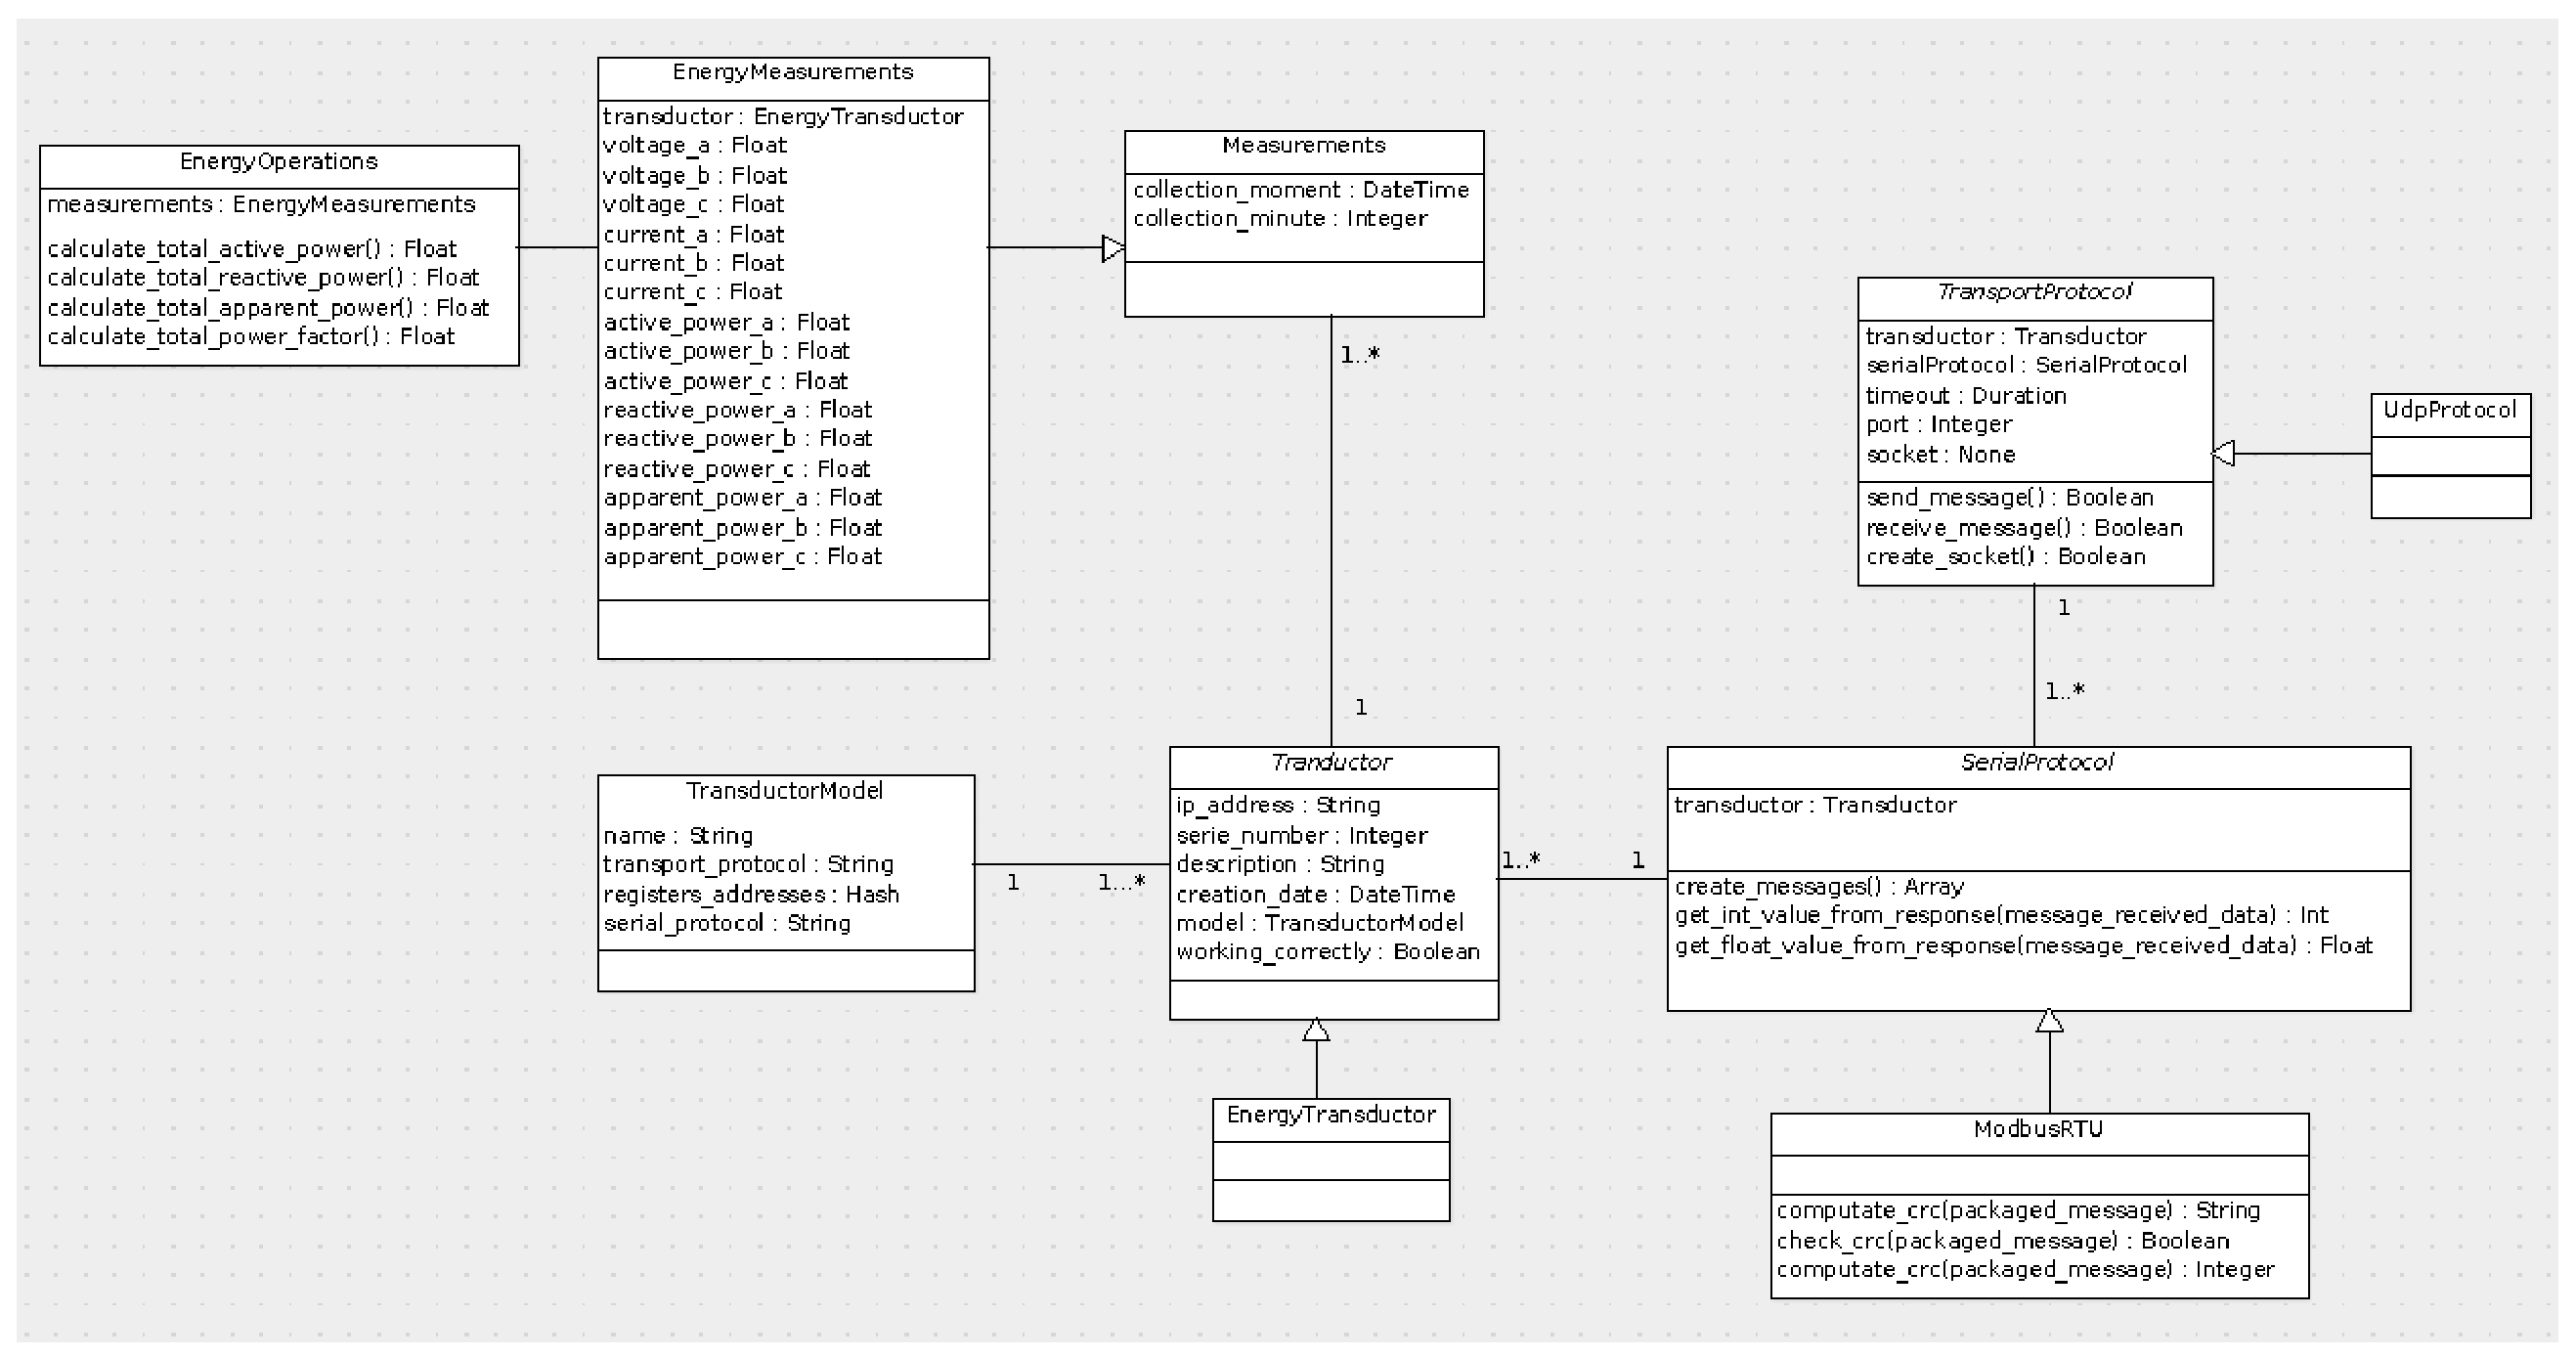
\includegraphics[scale=0.5,angle=90]{figuras/sprint05arq.eps}
    \caption{Arquitetura SME-UnB Sprint 05. Fonte: autor}
    \label{sprint05arq}
\end{figure}

Além das mudanças arquiteturais, foram implementadas e testadas as classes SerialProtocol, ModbusRTU e EnergyOperations. Obteve-se uma cobertura de 96\% ao fim da sprint, conforme ilustrado na figura \ref{cobertura02}.
\begin{figure}[!htpb]
    \centering
    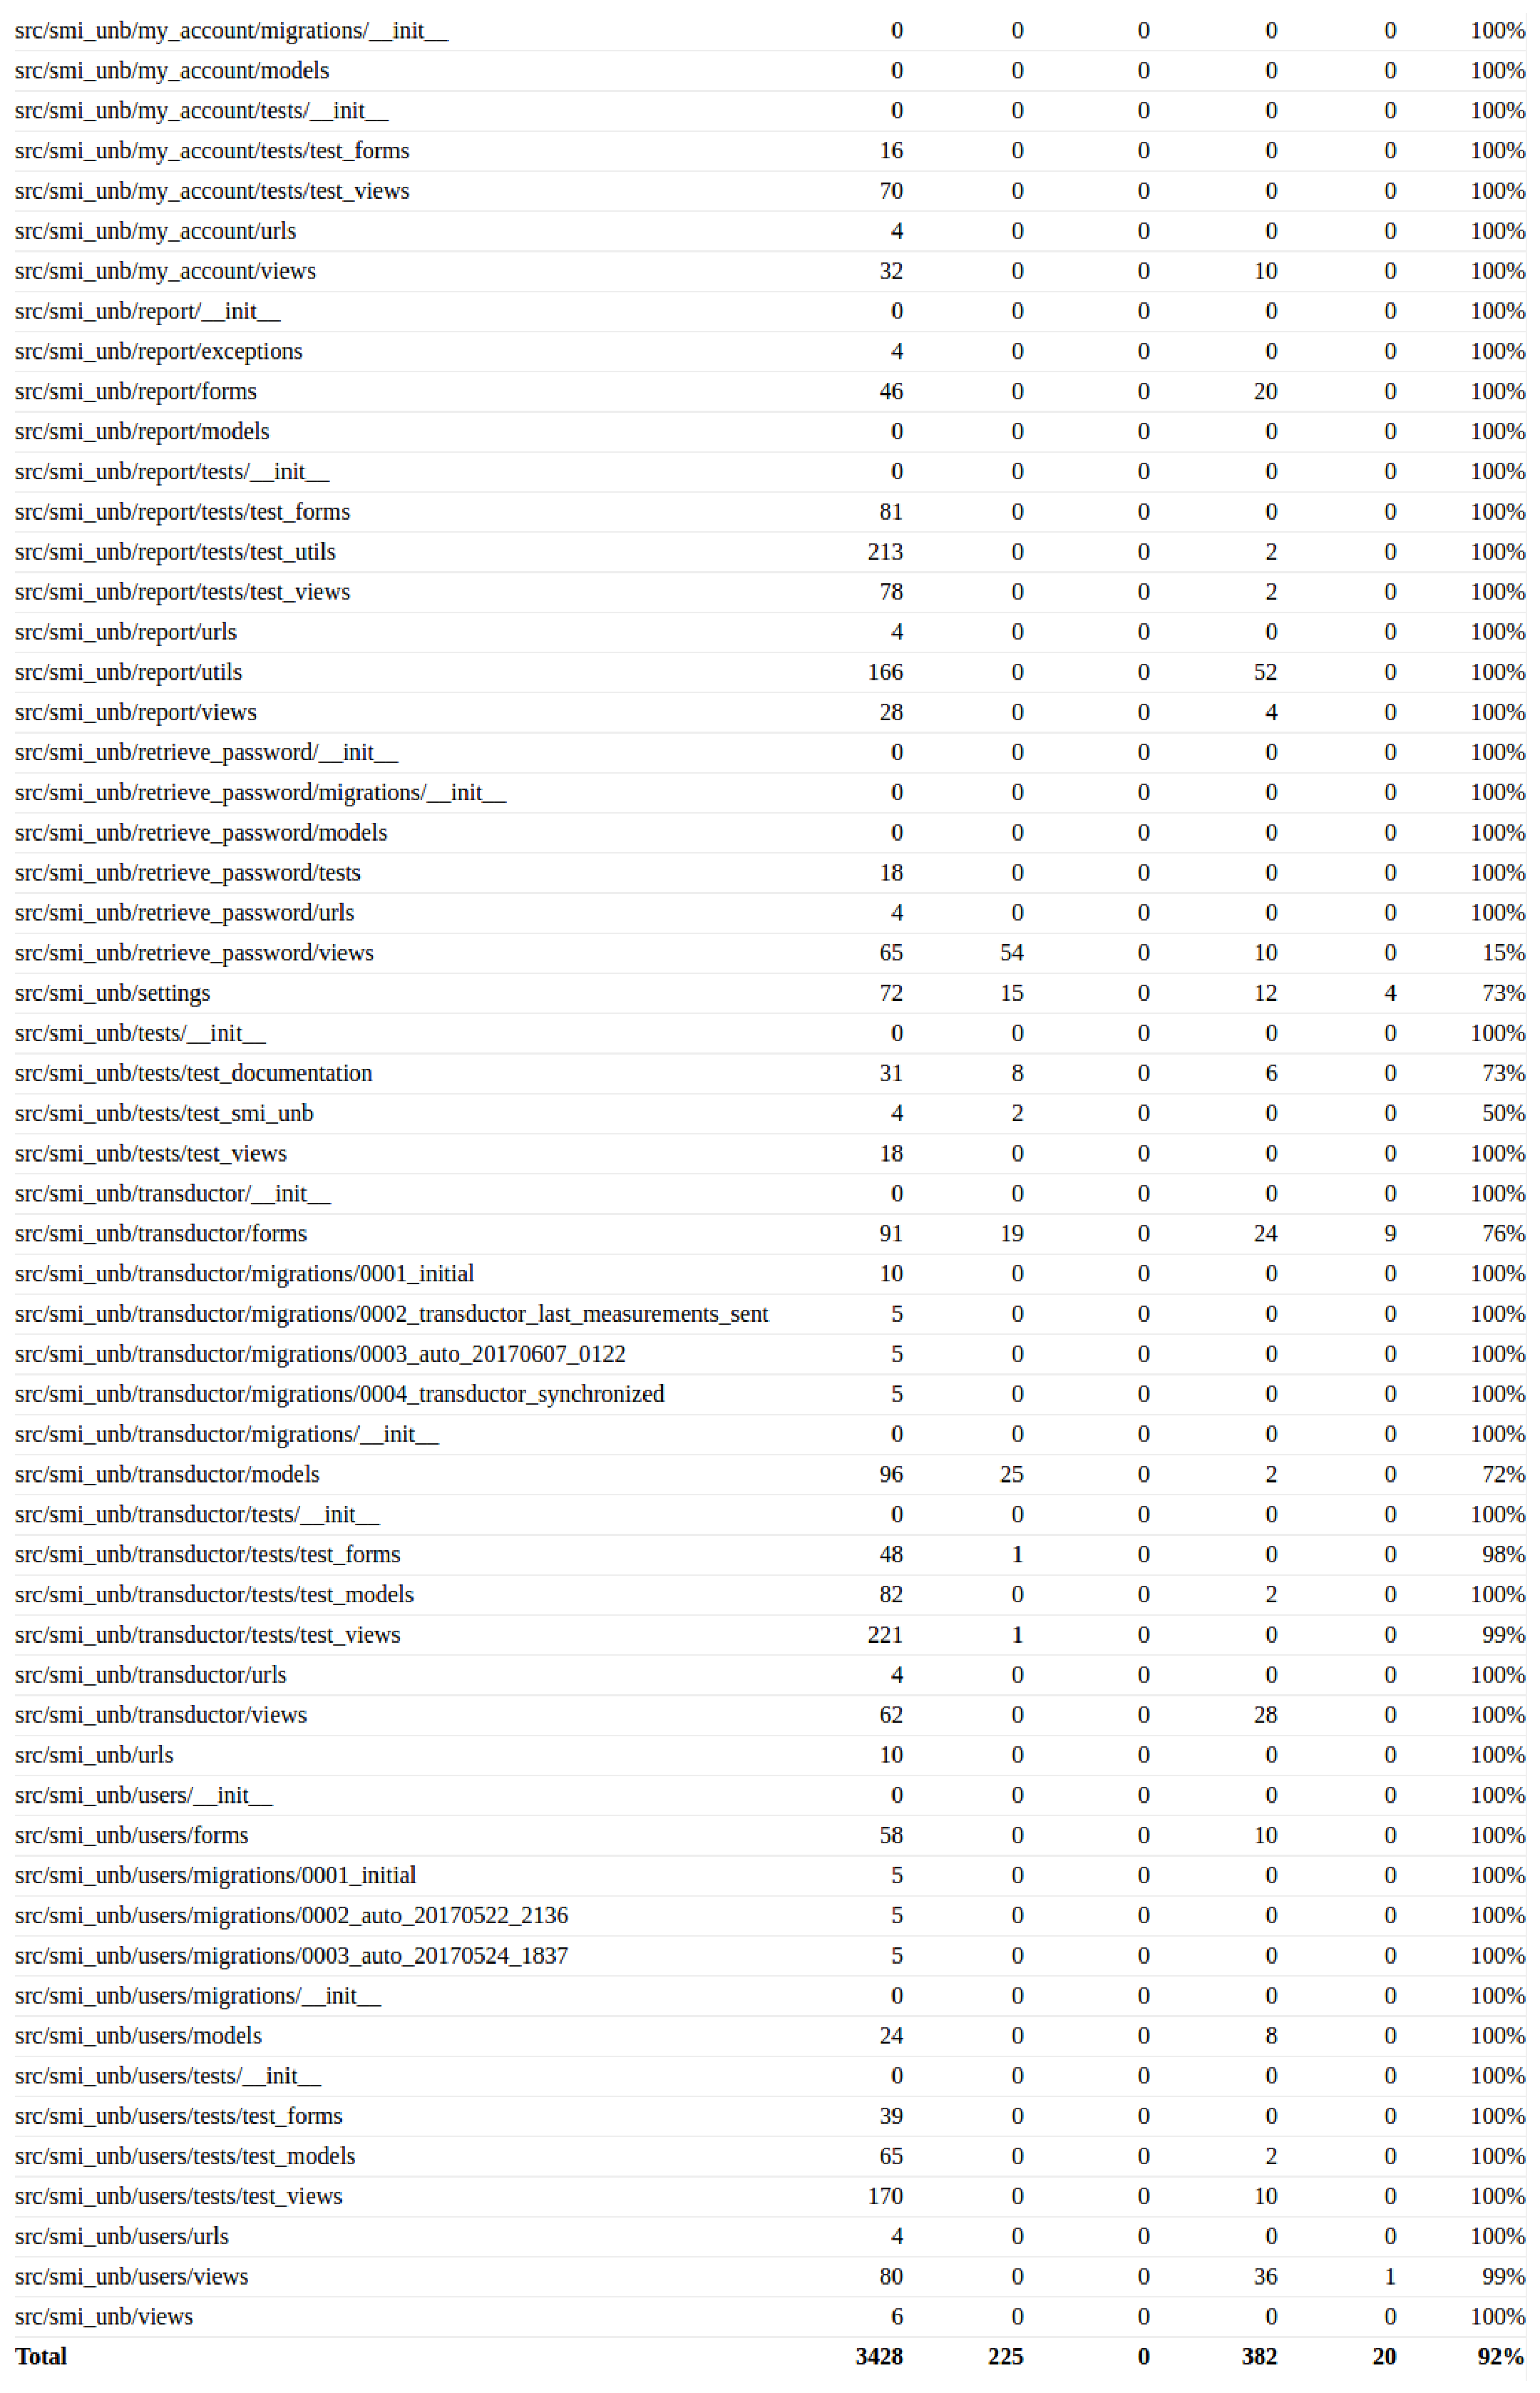
\includegraphics[keepaspectratio=true,scale=0.6]{figuras/cobertura02.eps}
    \caption{Cobertura Total de Código Sprint 05. Fonte: autor}
    \label{cobertura02}
\end{figure}

\section{Sprint 06 (03/10/2016 à 14/10/2016) - Protocolo de Transporte e Testes com \textit{Mock}}
Após implementado o protocolo serial, realizou-se o desenvolvimento do protocolo de transporte. Sua principal função é comunicar-se com o transdutor e tratar as questões referentes à \textit{timeout} e tentativas consecutivas de envio de requisições. Além disso, foram refatorados os testes do sistema utilizando \textit{Mocks}\footnote{\url{https://docs.python.org/3/library/unittest.mock.html}}, objetivando maior desempenho e unitariedade dos métodos. A figura \ref{exemplo_mock} ilustra um exemplo de teste da classe UdpProtocol utilizando \textit{Mock}. A cobertura de código, figura \ref{cobertura03}, não se alterou comparado à sprint anterior.

\begin{figure}[!htpb]
    \centering
    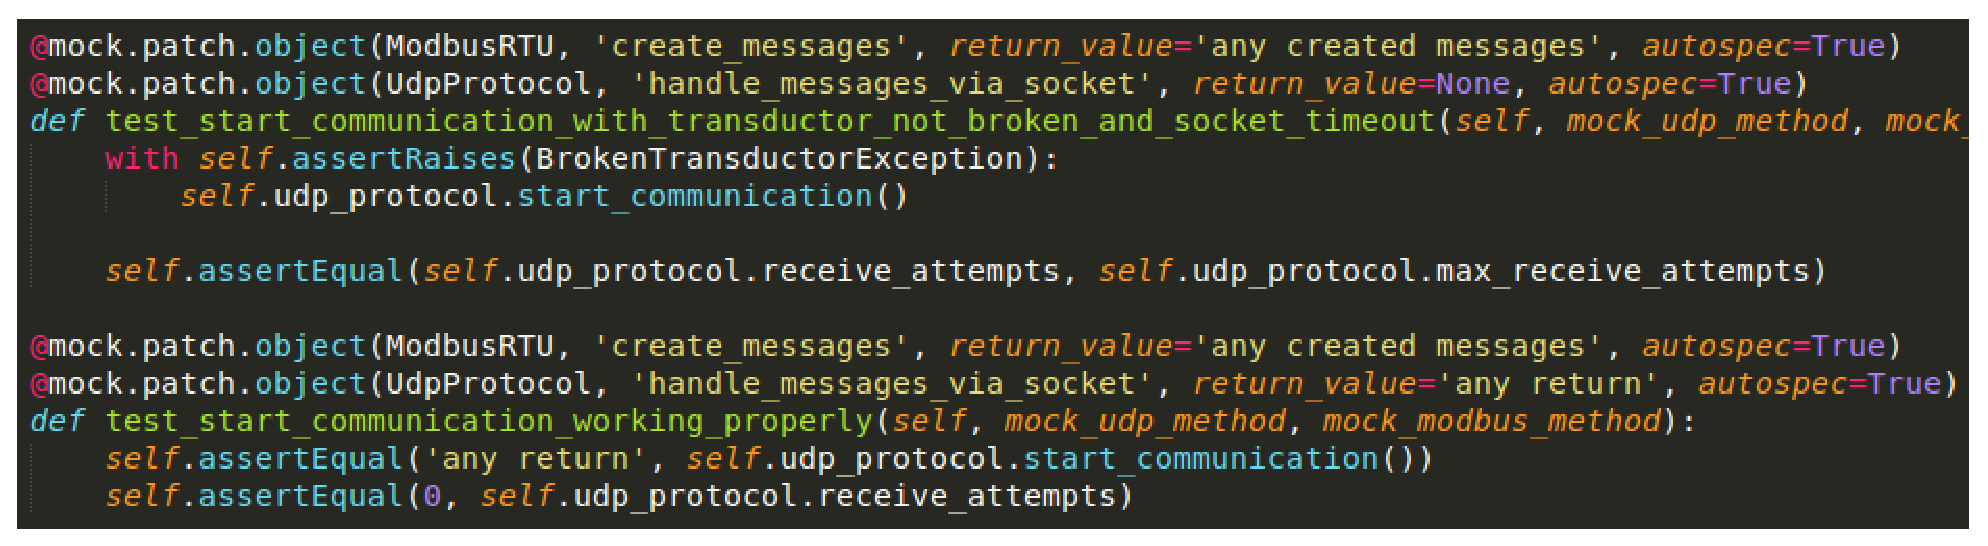
\includegraphics[keepaspectratio=true,scale=0.5]{figuras/exemplo_mock.eps}
    \caption{Exemplo de Teste utilizando \textit{Mock}. Fonte: autor}
    \label{exemplo_mock}
\end{figure}

\begin{figure}[!htpb]
    \centering
    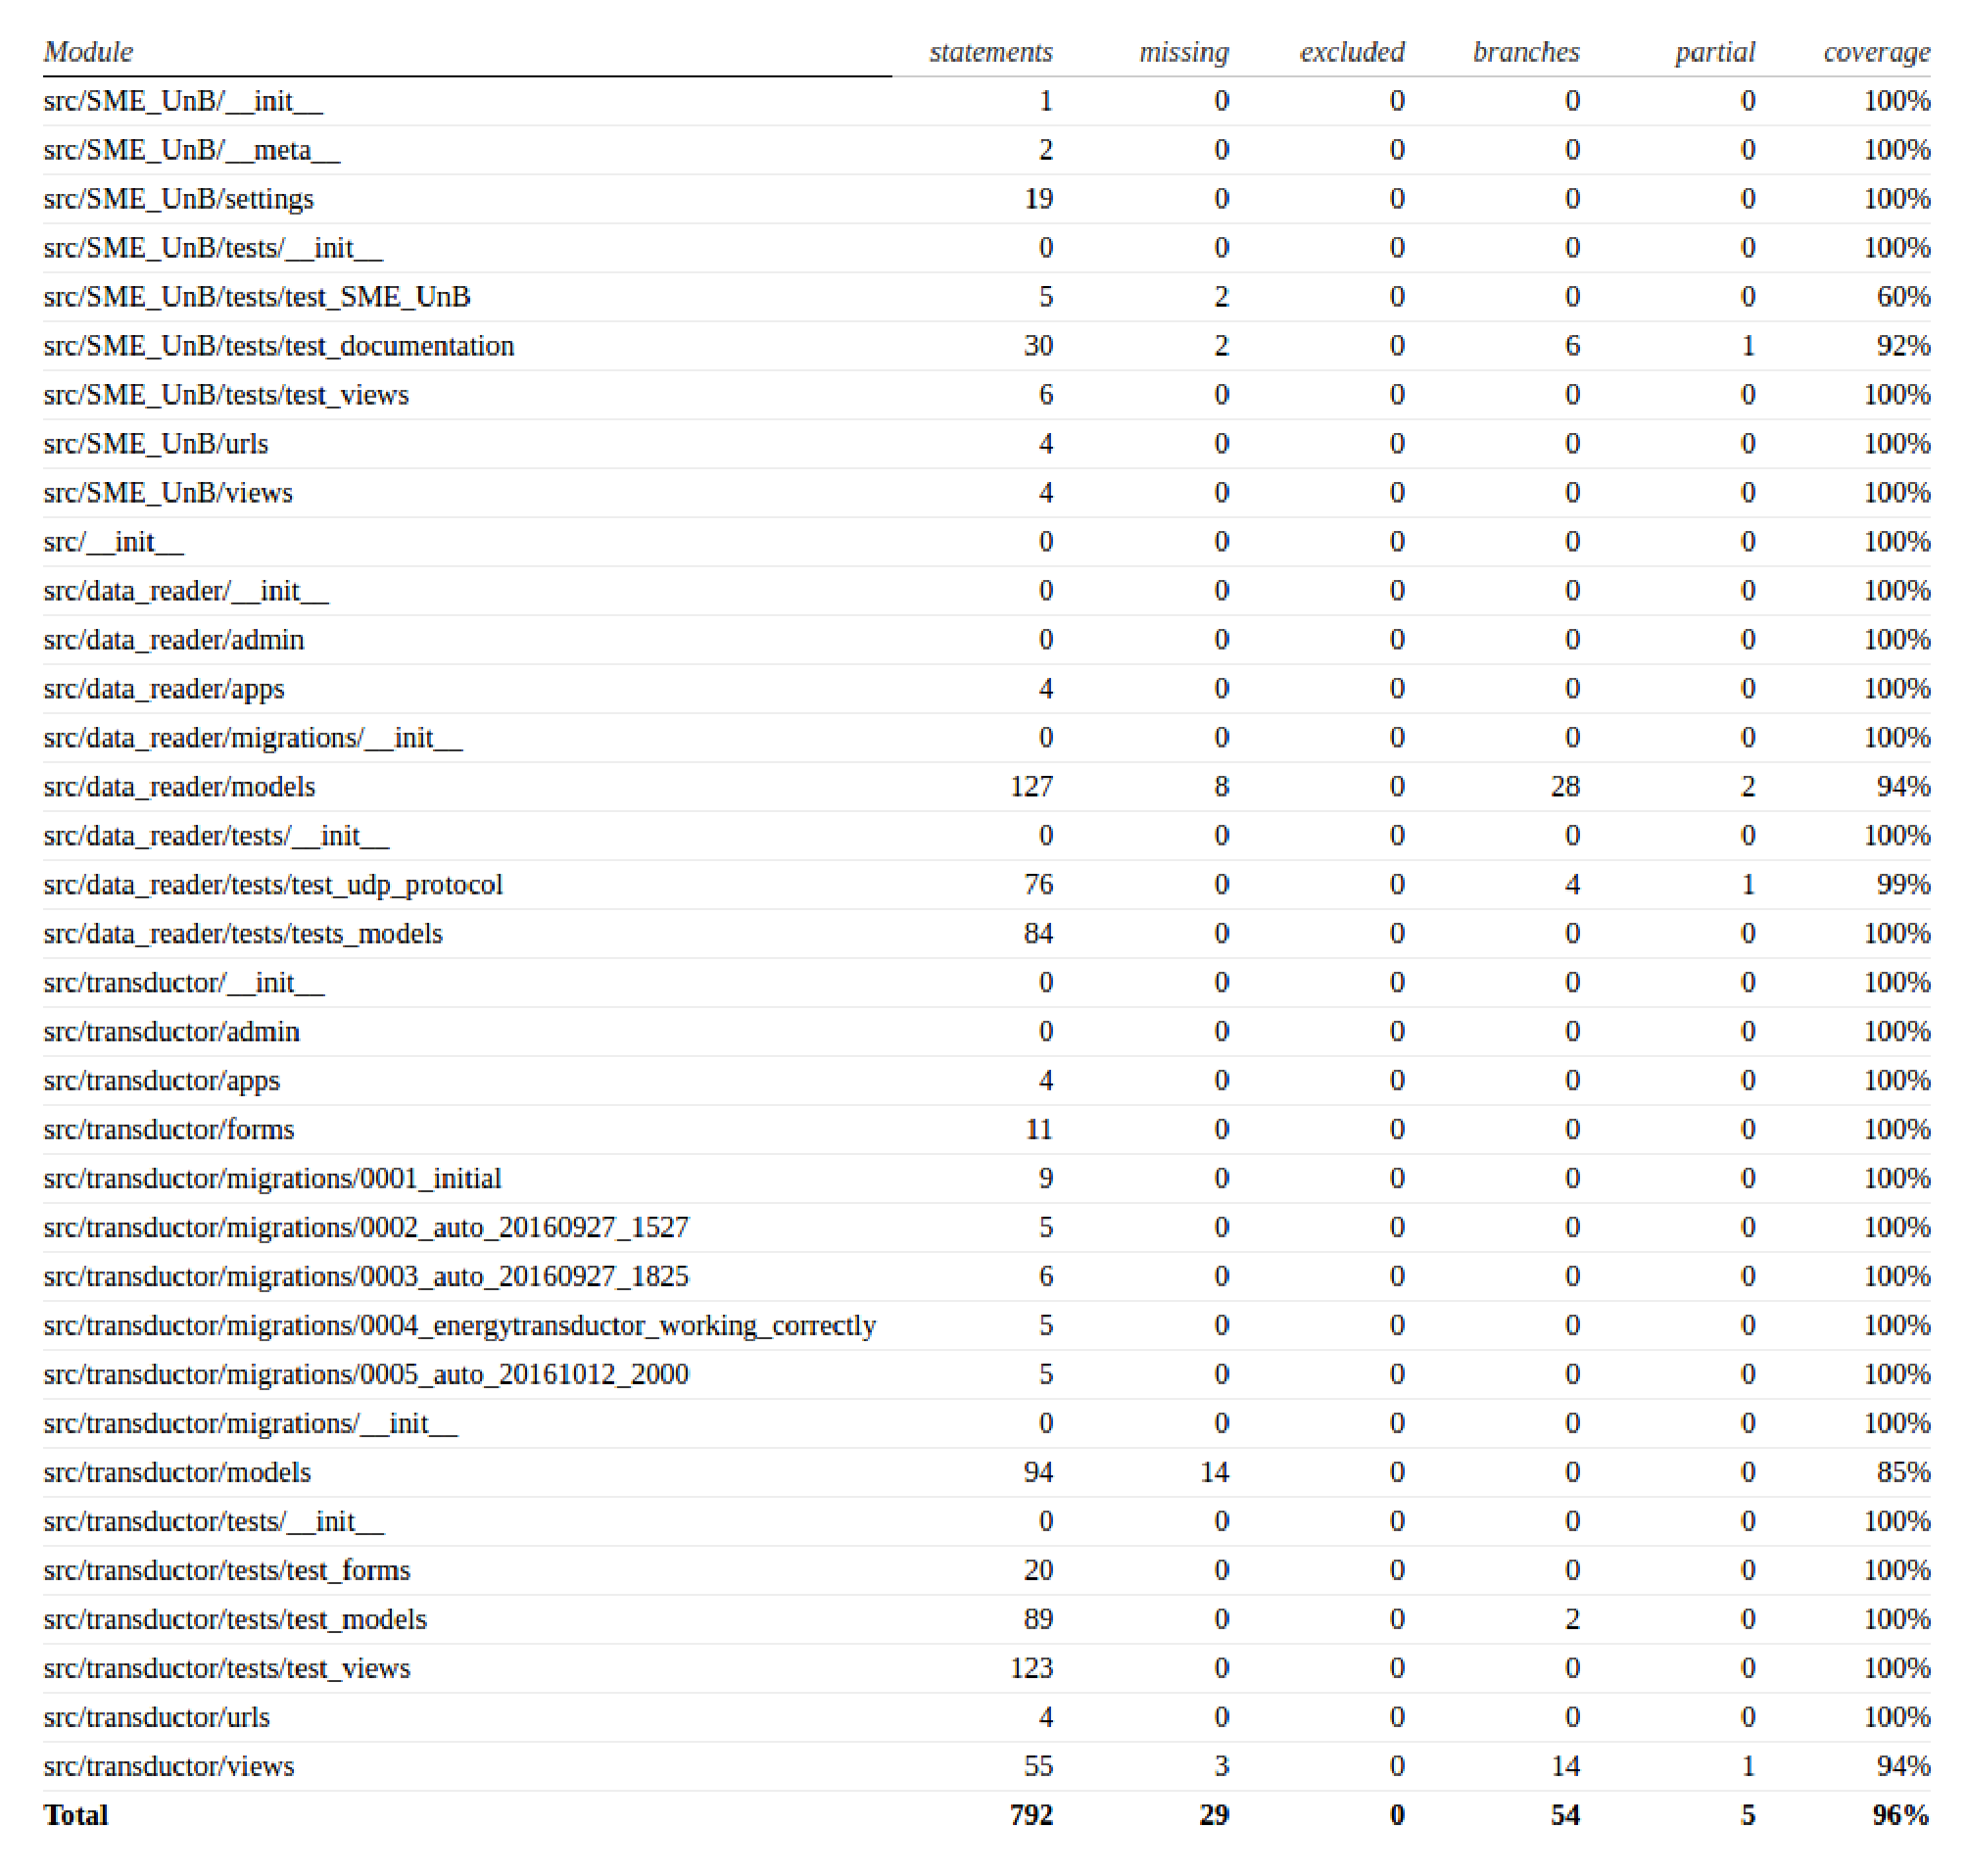
\includegraphics[keepaspectratio=true,scale=0.5]{figuras/cobertura03.eps}
    \caption{Cobertura Total de Código Sprint 06. Fonte: autor}
    \label{cobertura03}
\end{figure}

\section{Sprint 07 (17/10/2016 à 28/10/2016) - Gerenciador para Coleta de Dados}
Após implementar os protocolos de transporte e serial verificou-se a necessidade de uma classe que realizasse toda a comunicação dos mesmos, ou seja, desempenhasse a coleta das medições de cada transdutor. Essa classe foi definida como DataCollector e utiliza os princípios de \textit{threads}\footnote{\url{https://docs.python.org/2/library/threading.html}} para inicar ``simultaneamente'' a coleta de dados de todos os trandutores. A figura \ref{sprint07arq} ilustra a nova arquitetura gerada.

\begin{figure}[!htpb]
    \centering
    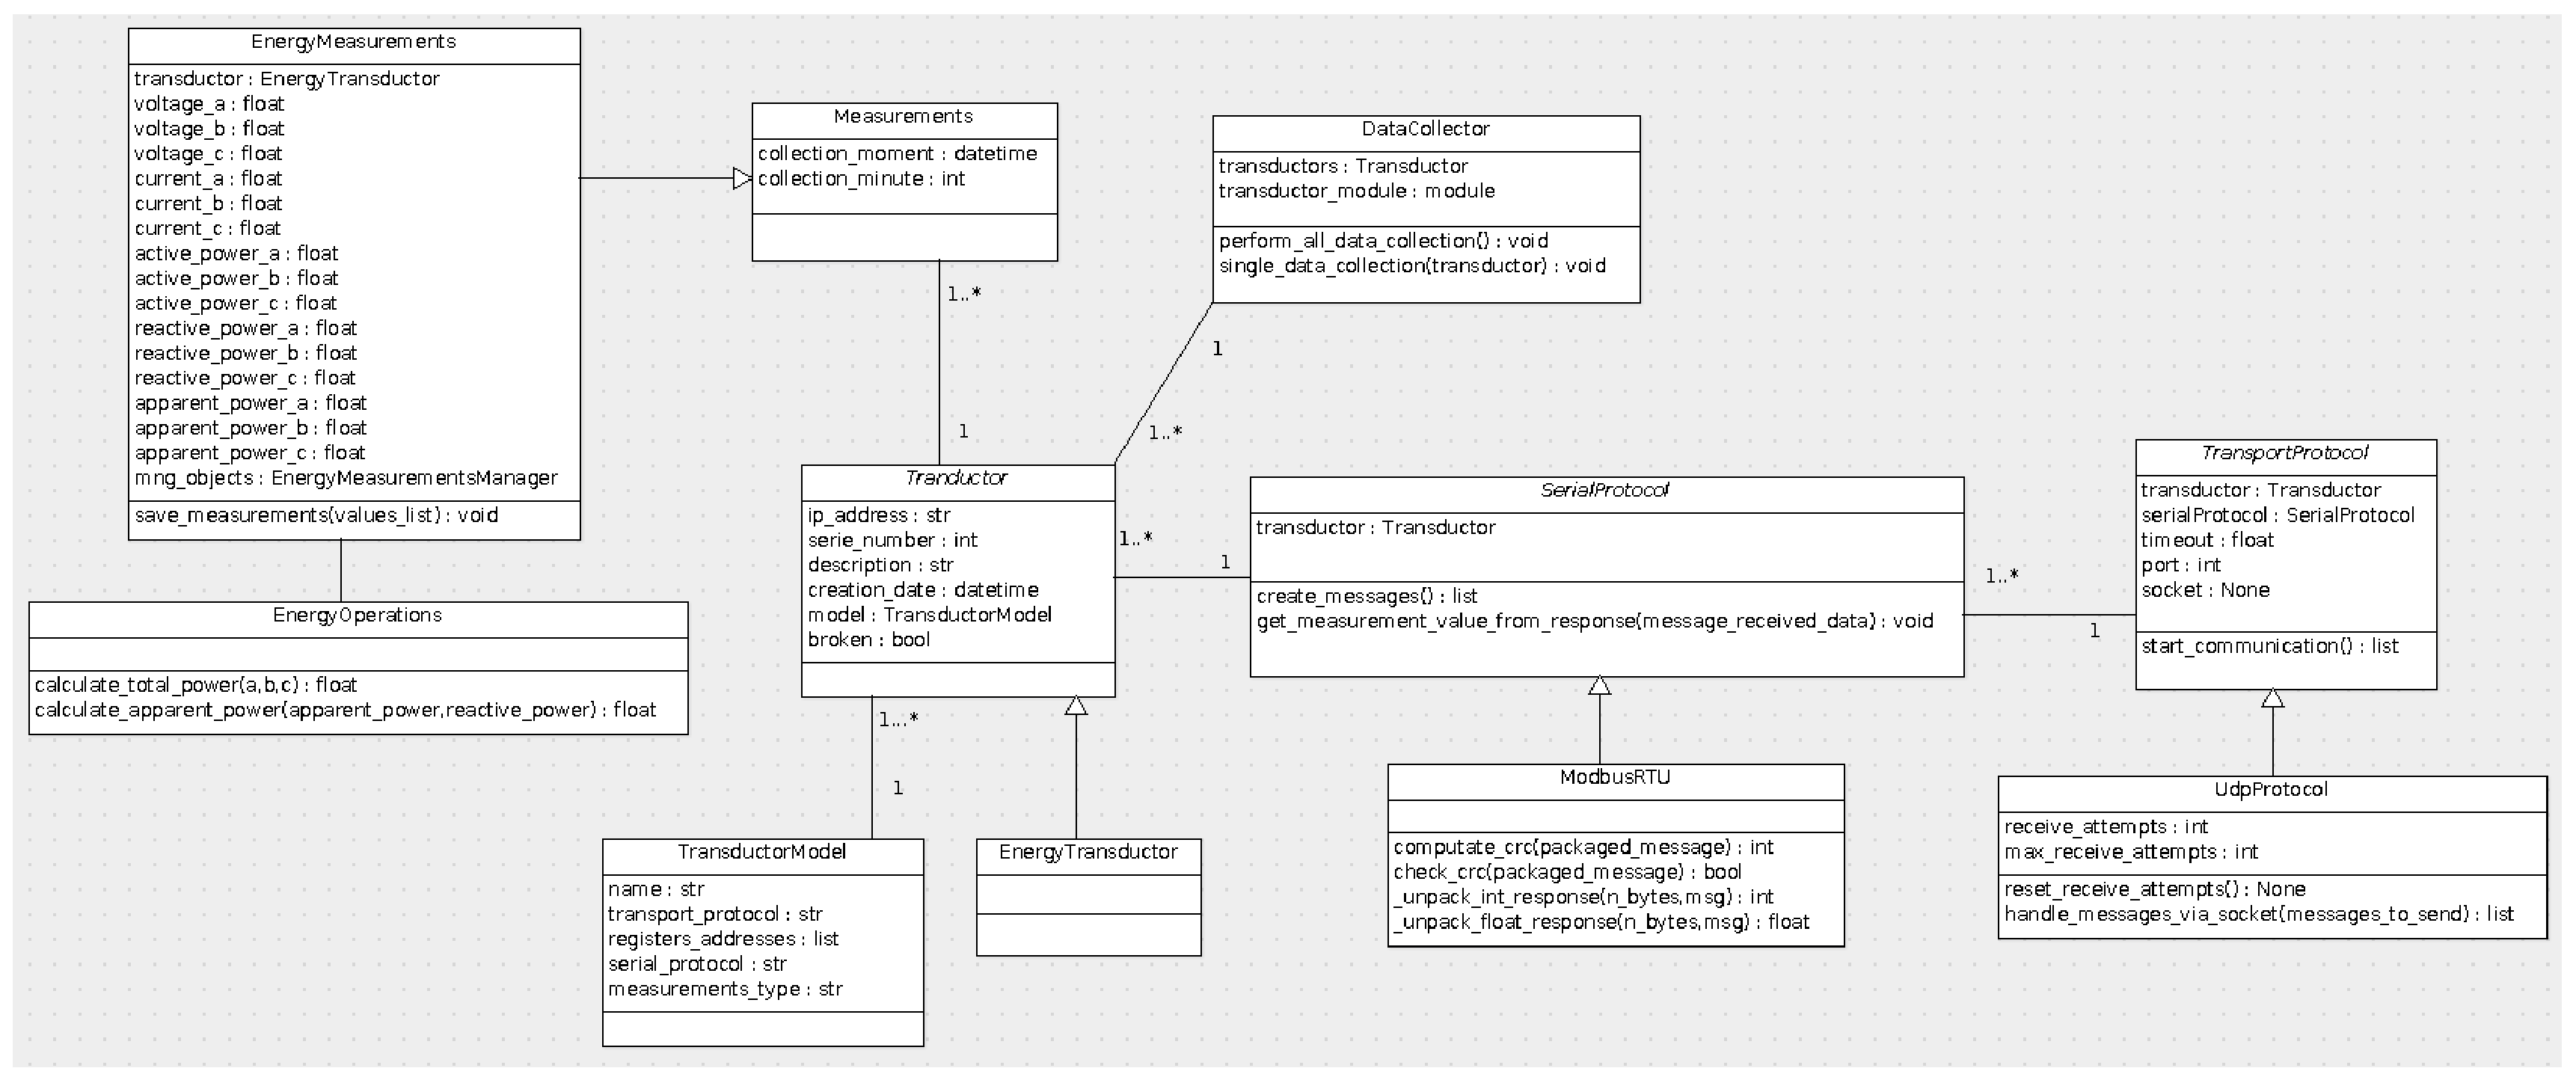
\includegraphics[scale=0.4,angle=90]{figuras/sprint07arq.eps}
    \caption{Arquitetura SME-UnB Sprint 07. Fonte: autor}
    \label{sprint07arq}
\end{figure}

A cobertura total de código obtida ao fim da sprint foi de 95\%, figura \ref{cobertura04}.
\begin{figure}[!htpb]
    \centering
    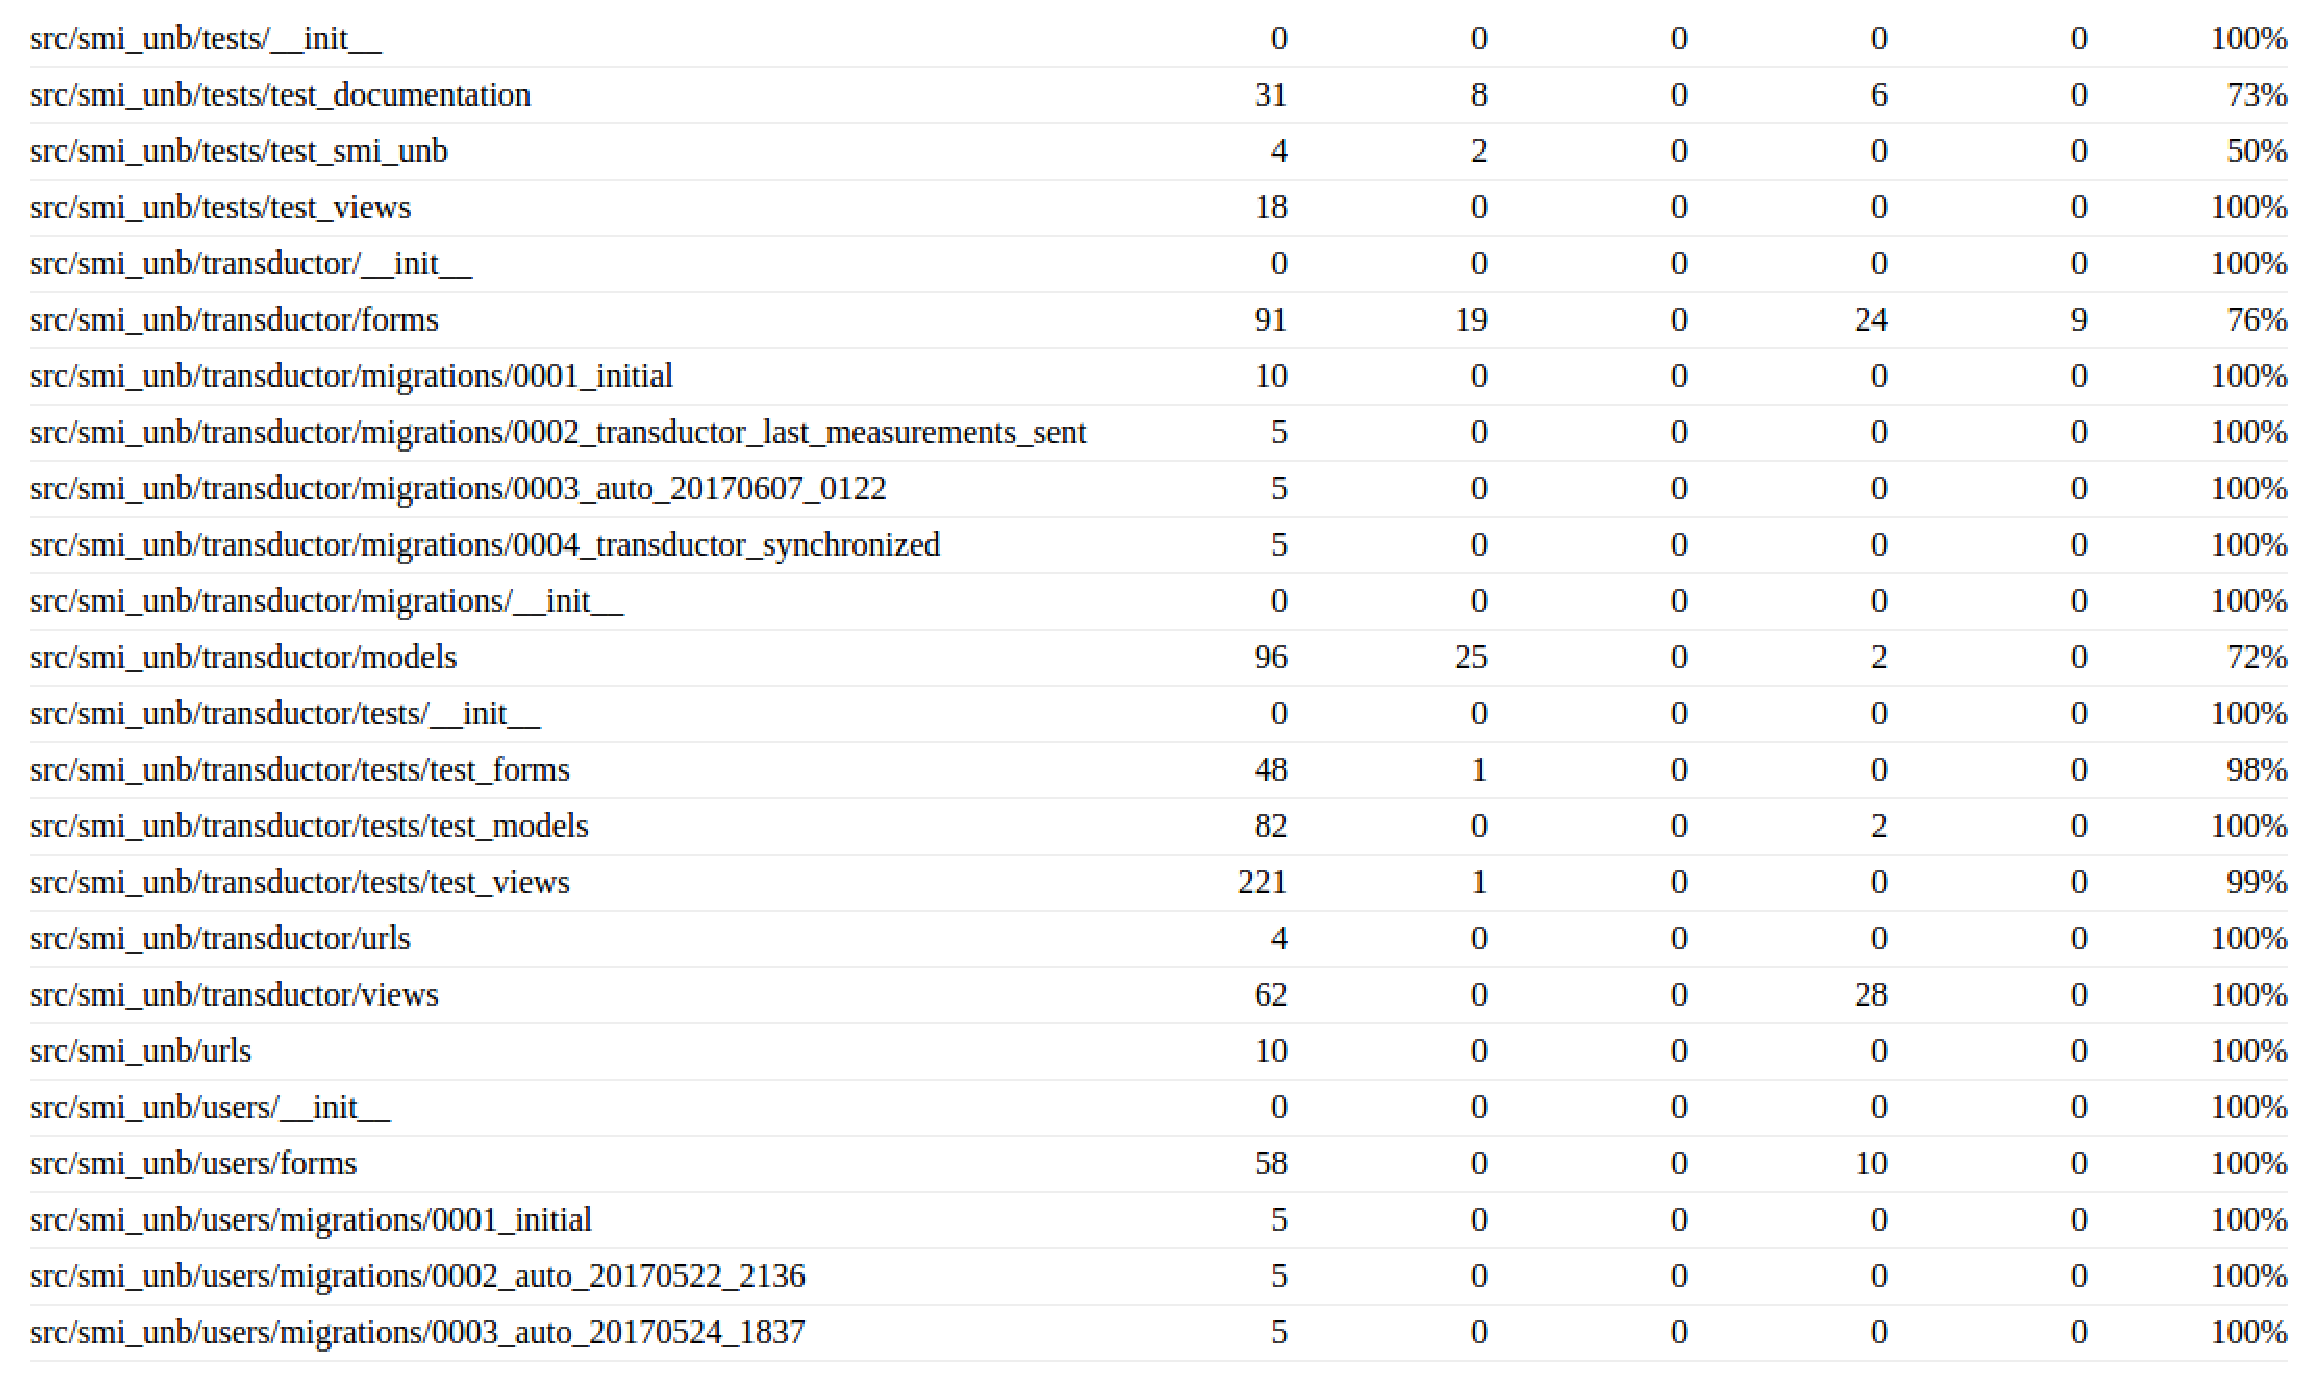
\includegraphics[keepaspectratio=true,scale=0.5]{figuras/cobertura04.eps}
    \caption{Cobertura Total de Código Sprint 07. Fonte: autor}
    \label{cobertura04}
\end{figure}

\section{Sprint 08 - \textit{Cron Job} e Integração Contínua}
Objetivando executar a coleta de dados de maneira temporizada, realizou-se a classe DataCollectCronJob, a qual foi programada para ser executado a cada 1 minuto. A arquitetura e cobertura de código finais da aplicação encontram-se nas figura \ref{sprint08arq} e \ref{cobertura05}.
\begin{figure}[!htpb]
    \centering
    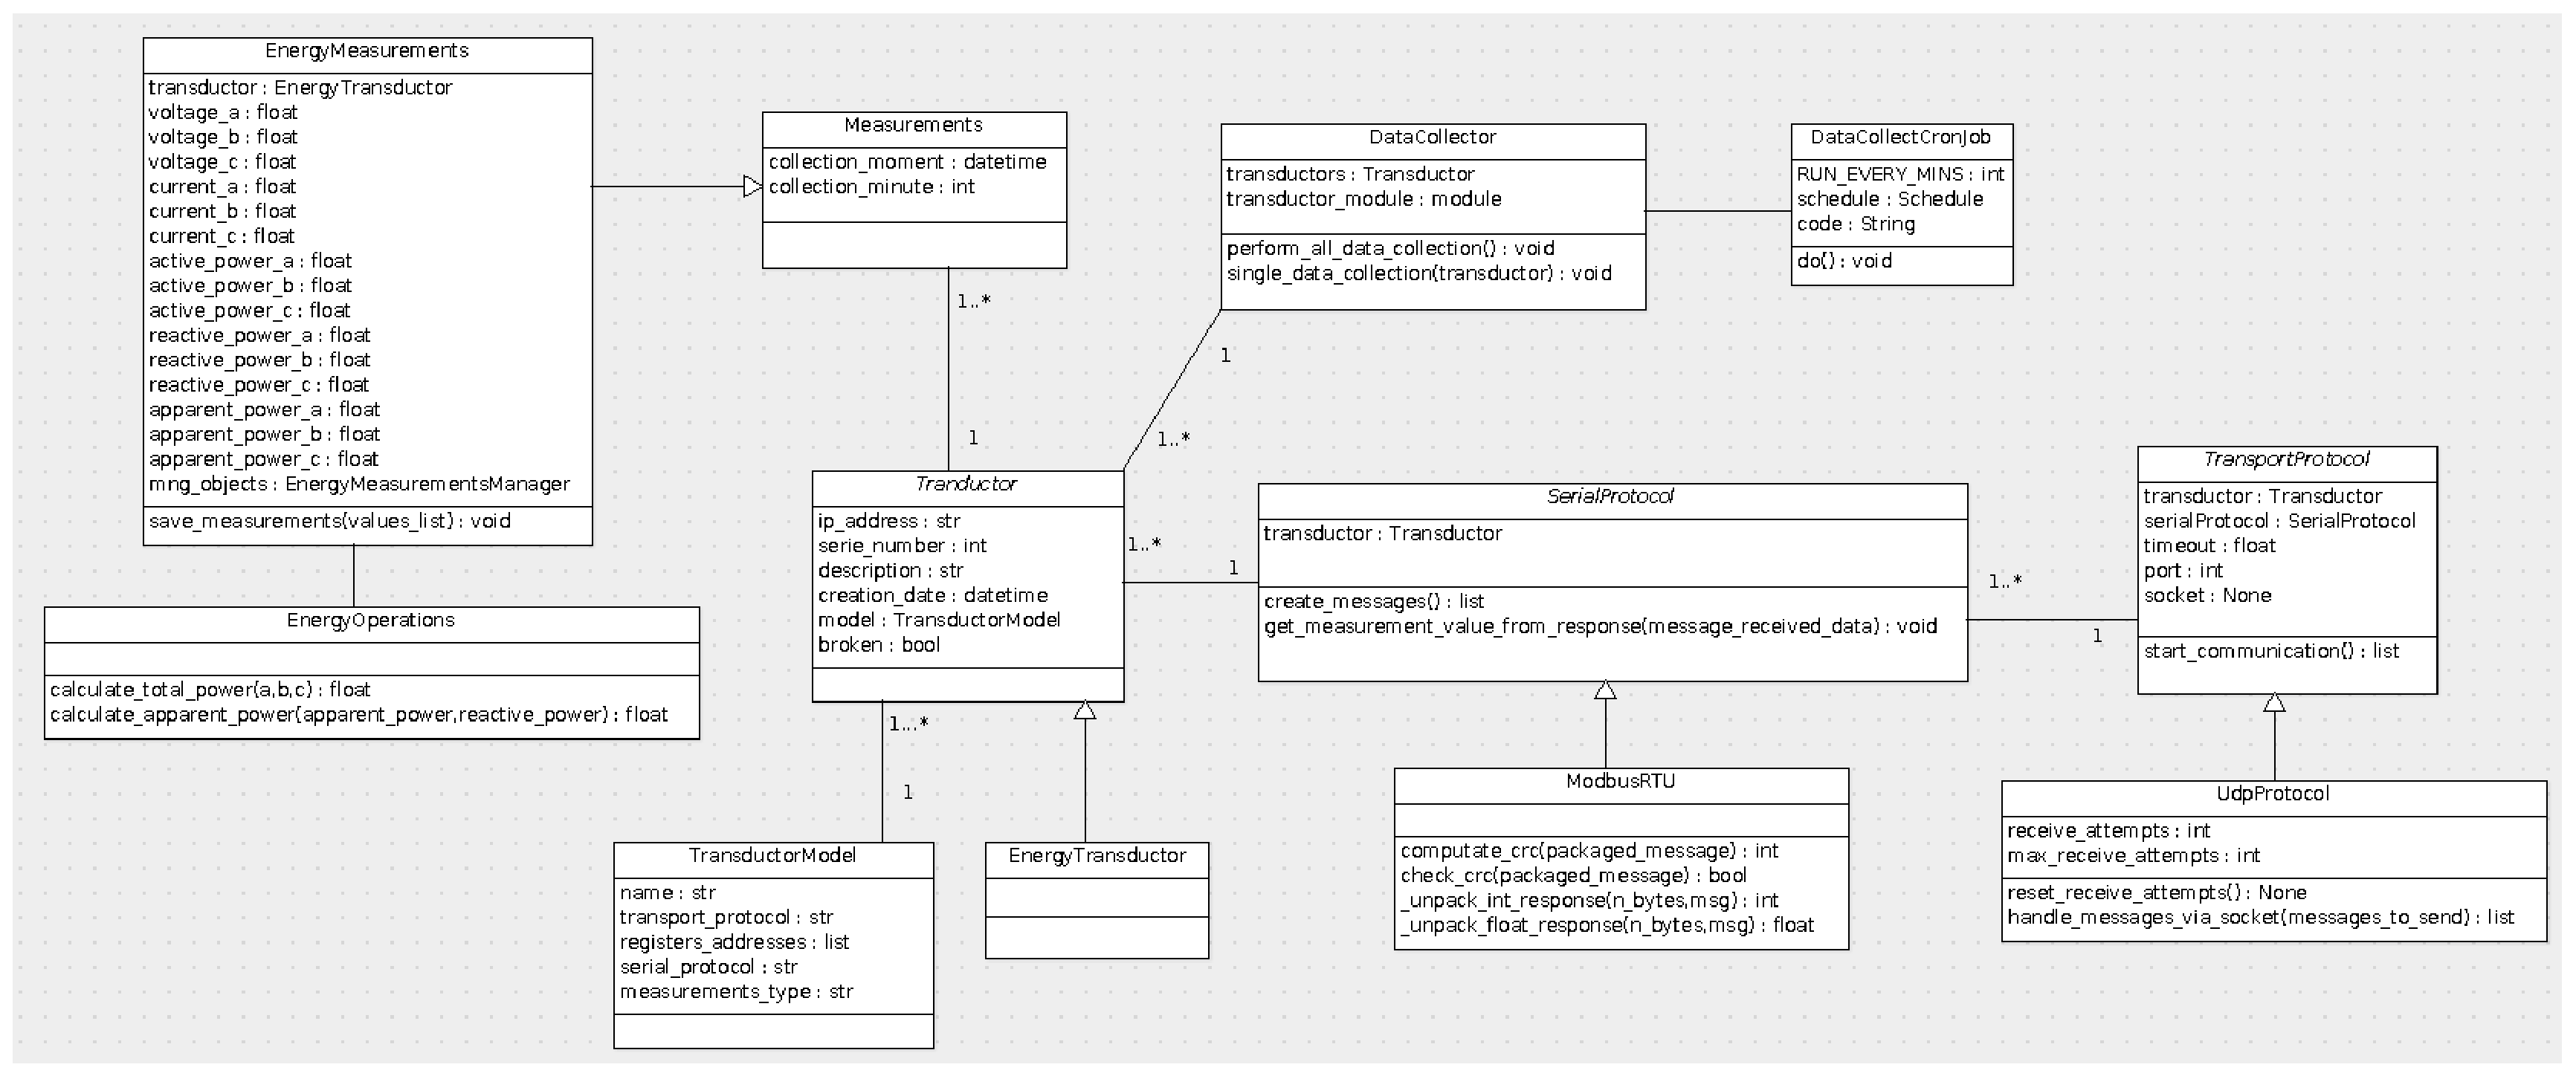
\includegraphics[scale=0.4,angle=90]{figuras/sprint08arq.eps}
    \caption{Arquitetura Final SME-UnB. Fonte: autor}
    \label{sprint08arq}
\end{figure}

\begin{figure}[!htpb]
    \centering
    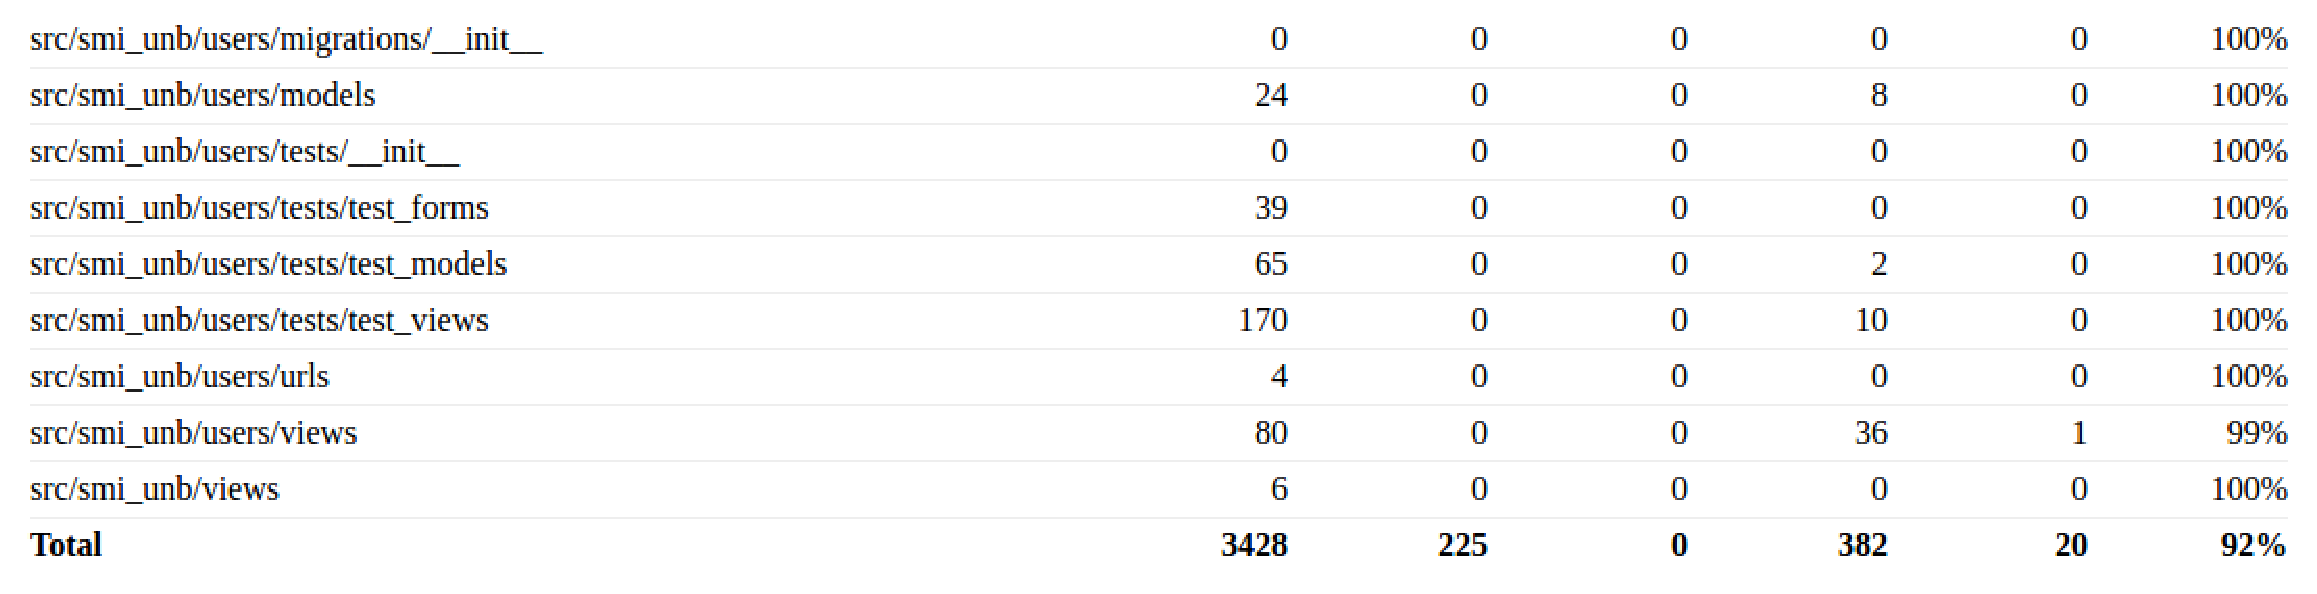
\includegraphics[keepaspectratio=true,scale=0.5]{figuras/cobertura05.eps}
    \caption{Cobertura Final de Código Obtida. Fonte: autor}
    \label{cobertura05}
\end{figure}